\chapter{The Standard Model of Particle Physics and supersymmetric models}
\label{chap:SMandSUSY}

%% Restart the numbering to make sure that this is definitely page #1!
\pagenumbering{arabic}

%% Note that the citations in this chapter use the journal and
%% arXiv keys: I used the SLAC-SPIRES online BibTeX retriever
%% to build my bibliography. There are also quite a few non-standard
%% macros, which come from my personal collection. You can have them
%% if you want, or I might get round to properly releasing them at
%% some point myself.

\chapterquote{If I could remember the names of these particles, I would have been a botanist.}%
{Enrico Fermi, 1901--1954}

\section{Prelude: Dirac, Weyl and Majorana Spinors}
\label{sec:diracweyl}

Supersymmetry is built upon the arguably less familiar Weyl and Majorana type fermions, rather than the 4-component Dirac fermion. Matter fields in supersymmetric theories are placed in an \textit{irreducible representation} of the supersymmetry algebra called chiral supermultiplets, each one containing a Weyl fermion. Hence it is useful to exploit a representation of the Lorentz group that is irreducible - the Weyl spinor. This avoids the unnecessary introduction of extra operators on the reducible Dirac representation throughout the theory that can potentially complicate matters. Since parity is not a fundamental symmetry of the group, left and right-handed fermions must be treated differently, with different quantum numbers under the Standard Model gauge group. For example, left-handed fermions participate in the weak interaction, whereas right-handed fields are singlets under the electroweak gauge group, described by $\SUgroup{2} \times \Ugroup{1}_Y$.

The dynamics of spin-1/2 fermions in the Standard Model are famously described by the Dirac equation, with Lagrangian (in natural units where $\hbar=c=1$):
\begin{equation}
\mathcal{L}_{Dirac}=\overline{\Psi}(i\gamma^{\mu}\partial_{\mu}-m)\Psi,
\end{equation}
where $\Psi$ is the 4-component Dirac spinor, also called a bispinor. Here, and throughout this thesis, we use the flat spacetime metric in the \textit{mostly negative} regime $\eta_{\mu\nu}$= diag(1,-1,-1,-1). The $\gamma^{\mu}$, where $\mu=\{0,1,2,3\}$, are the 4x4 Dirac matrices and the field has the adjoint $\overline{\Psi}=\gamma^{0}\Psi^{\dagger}$. The Dirac field is massive coming from the term $-m\bar{\psi}\psi$, however one cannot include this term in the Standard Model and simultaneously preserve gauge invariance. Instead in the Standard Model, fermions start off massless and subsequently acquire their mass through the Higgs mechanism. The Dirac spinor can then be written in terms of two-component objects, a left-handed and right-handed Weyl spinor $\eta$ and $\chi^{\dagger}$ respectively:
\begin{equation}
\Psi=\begin{pmatrix}
\eta_{\alpha} \\
\chi^{\dagger \dot{\alpha}}
\end{pmatrix},\quad
\overline{\Psi}=\begin{pmatrix}
\chi^{\alpha} &
\eta^{\dagger}_{\dot{\alpha}}
\end{pmatrix},
\end{equation}
with spinor indices $\alpha=1,2$ and $\dot{\alpha}=1,2$ counting over the complex degrees of freedom. One can define operators that project the left and right-handed states through the $\gamma^{5}$ matrix, written in the 2 x 2 block matrix representation as:
\begin{equation}
P_{L}=\frac{1-\gamma_{5}}{2},\quad P_{R}=\frac{1+\gamma_{5}}{2},\quad \gamma_{5}=\begin{pmatrix}
\textbf{-1} & \textbf{0} \\
\textbf{0} & \textbf{1} \\
\end{pmatrix},
\end{equation}
where $\gamma^5$ is in the \textit{Weyl} or \textit{chiral} basis. Acting upon the Dirac spinor projects the necessary state:
\begin{equation}
\Psi_{L}=P_{L}\Psi=\begin{pmatrix}
\eta_{\alpha} \\
0
\end{pmatrix}
,\quad \Psi_{R}=P_{R}\Psi=\begin{pmatrix}
0 \\
\chi^{\dagger \dot{\alpha}}
\end{pmatrix},
\end{equation}
so clearly a Dirac spinor satisfies $\Psi=\Psi_{L}+\Psi_{R}$. Obviously, $\Psi_{L}$ and $\Psi_{R}$ are eigenstates of helicity, which is not a Lorentz-invariant quantity (only in the massless fermion case). Hence we define them as eigenstates of $\gamma^5$ known as the \textit{chirality} of the left or right-handed field, whose eigenvalues are $\pm 1$. Since the left and right-handed spinors transform as separate and distinct representations of the Lorentz group, this shows that the Dirac spinor does indeed form a reducible representation. Since Weyl fermions are 2-component objects, their dynamics are instead represented using the 2 x 2 Pauli matrices:
\begin{equation}
\mathcal{L}_{Dirac}=i\eta^{\dagger}\overline{\sigma}^{\mu}\partial_{\mu}\eta+i\chi^{\dagger}\overline{\sigma}^{\mu}\partial_{\mu}\chi-m(\eta \chi + \eta^{\dagger} \chi^{\dagger}),
\end{equation}
where we have suppressed explicit dependence on the spinor indices. The final two terms also clearly show that massive fermions break chiral symmetry explicitly.

Demanding that $\chi=\eta$, one can construct a Majorana-type fermion:
\begin{equation}
\Psi_{Majorana}=\begin{pmatrix}
\eta_{\alpha} \\
\eta^{\dagger \dot{\alpha}}
\end{pmatrix}.
\end{equation}
These will become important in supersymmetric gauge theories, which place the gauge bosons and their superpartners, the \textit{gauginos} into irreducible representations called gauge supermultiplets. Since the quantum numbers of the partner gauginos are identical to their corresponding gauge boson, they also must be their own antiparticle - and hence Majorana fermions. This is especially applicable to models of dark matter - of which the supersymmetric candidate is indeed Majorana. 
A Majorana fermion has the corresponding Lagrangian:
 \begin{equation}
\mathcal{L}_{Majorana}=i\eta^{\dagger}\overline{\sigma}^{\mu}\partial_{\mu}\eta-\frac{1}{2}m(\eta\eta+\eta^{\dagger}\eta^{\dagger}).
 \end{equation}

\section{The Standard Model: Matter and Gauge Fields}
\label{sec:sm}
The Standard Model (\acrshort{sm}) \cite{RN291,RN288,RN294,RN299} is a non-Abelian Yang-Mills theory based on three continuous symmetry groups that transform independently, denoted by the direct product $\SUgroup{3}_{C} \times \SUgroup{2}_{L} \times \Ugroup{1}_{Y}$. Respectively these represent the strong (colour) interaction, weak isospin and weak hypercharge gauge groups. It is a relativistic quantum field theory and so respects Poincar\'{e} symmetry. This comprises invariance under space-time translations, rotations and inertial reference frames, of which the last two form the Lorentz subgroup.

The Standard Model requires invariance under \textit{local transformations}, which forces one to introduce a set of gauge interactions with the matter fields, completely determined by the local gauge symmetry.
For a set of transforming gauge fields $A^a_{\mu}$ where the Roman alphabet indices represent the gauge degrees of freedom, one can maintain gauge invariance in the theory with covariant derivatives:
\begin{equation}
\partial_{\mu}\rightarrow D_{\mu}=\partial_{\mu}+igA^{a}_{\mu}T^{a}.
\end{equation}
Sums over repeated indices are implied. The generators $T^a$ depend on the group representation of the matter field to which they are coupled. For the $\Ugroup{1}_{Y}$ there is a single hypercharge operator, for $\SUgroup{2}$ there are the 3 Pauli matrices $\sigma^{i} (i=1,2,3)$, and the 8 Gell-Mann matrices $\lambda^{j} (j=1,2,...8)$ for $\SUgroup{3}_{C}$. The full matter Lagrangian is then identified as:
\begin{equation}
\mathcal{L}_{Matter}=i\overline{L}\gamma^{\mu}D_{\mu}L+i\overline{Q}\gamma^{\mu}D_{\mu}Q+i\overline{u}\gamma^{\mu}D_{\mu}u+i\overline{d}\gamma^{\mu}D_{\mu}d+i\overline{e}\gamma^{\mu}D_{\mu}e,
\end{equation}
with the fields defined in Table \ref{tab:SMcontent}. The matter fields reside in one particular representation of the gauge group called the \textit{fundamental representation}, however the gauge fields are in the \textit{adjoint representation}, that is, they are defined through the structure constants:
\begin{equation}
(T^a)_{bc}=-if^{abc},\quad a,b,c \in (1,...,N^2-1).
\end{equation}
In general, if $N$ is the dimension of the symmetry group, an \SUgroup{N} group will contain $N^2-1$ degrees of freedom. For example, for the $\SUgroup{3}_{C}$ group, this implies the existence of 8 gluons. The basis for the generators are arbitrary, but are chosen in this representation such that they satisfy:
\begin{equation}
Tr(T^{a}T^{b})=\frac{\delta^{ab}}{2}.
\end{equation}
In addition to the matter fields, gauge fields for each symmetry group have gauge-invariant kinetic terms:
\begin{equation}
\mathcal{L}_{Gauge}=-\frac{1}{4}G^a_{\mu\nu}G^{a\mu\nu}-\frac{1}{4}W^a_{\mu\nu}W^{a\mu\nu}-\frac{1}{4}B_{\mu\nu}B^{\mu\nu},
\end{equation}
given the gauge field strength terms $F^a_{\mu\nu}=\partial_{\mu}A^a_{\nu}-\partial_{\nu}A^a_{\mu}-gf^{abc}A^b_{\mu}A^c_{\nu}$. Non-abelian gauge fields for which the generators do not commute lead to gauge self-interactions, particularly important for such phenomena as \acrshort{qcd} asymptotic freedom. Note that gauge invariance forbids terms like $\frac{1}{2}m^2 A^{\mu}A_{\mu}$, eg. the mass of the photon, and furthermore gauge bosons remain massless without an additional mechanism.

Finally, one can recognize that these are not the only combination of SM fields that produce a gauge-invariant quantity. The matter fields can also be coupled to the Higgs doublet $\Phi$ through the Yukawa-Higgs interaction:
\begin{equation}
\mathcal{L}_{Yukawa}=-y_{u}\overline{Q}\Phi^{\dagger}u-y_{d}\overline{Q}\Phi d-y_{e}\overline{L}\Phi e + h.c.,
\end{equation}
where $y_{u,d,e}$ are 3x3 Yukawa matrices in family space.

\begin{table}[h]
\centering
\caption[Standard Model matter and gauge field contents.]{The Standard Model matter and gauge field contents with associated quantum numbers for each field. Quarks and Leptons both have 3 families that transform the same under the SM gauge group.}
\label{tab:SMcontent}
\begin{tabular}{|c|c|c|c|}
\hline
\multicolumn{2}{|c|}{Name}                         &                                         & $\SUgroup{3}_{C},\SUgroup{2}_{L},\Ugroup{1}_{Y}$        \\ \hline
\multicolumn{4}{|c|}{Matter Fields (Spin-1/2)}                      \\ \hline
\multirow{3}{*}{Quarks (3 Gen.)}       & $Q$  & $\left ( u_{L} ~~ d_{L} \right )$   &   (\textbf{3},\textbf{2},$\frac{1}{6}$)      \\ \cline{2-4} 
                              & $\overline{u}$  & $u^{\dagger}_{R}$    & (\textbf{$\overline{3}$},\textbf{1},$-\frac{2}{3}$)            \\ \cline{2-4} 
                              & $\overline{d}$  & $d^{\dagger}_{R}$    &   (\textbf{$\overline{3}$},\textbf{1},$\frac{1}{3}$)          \\ \hline
\multirow{2}{*}{Leptons (3 Gen.)}      & $L$        & $\left ( \nu_{L} ~~ e_{L} \right )$    & (\textbf{1},\textbf{2},$-\frac{1}{2}$)            \\ \cline{2-4} 
                              & $\overline{e}$   & $e^{\dagger}_{R}$       &       (\textbf{1},\textbf{1},1)       \\ \hline
\multicolumn{4}{|c|}{Gauge Fields (Spin-1)}                         \\ \hline
\multicolumn{2}{|c|}{B Boson}           &  $B$          & (\textbf{1},\textbf{1},0)         \\ \hline
\multicolumn{2}{|c|}{W Bosons}          &  $W$          & (\textbf{1},\textbf{3},0)            \\ \hline
\multicolumn{2}{|c|}{Gluons}          &  $g$          &  (\textbf{8},\textbf{1},0)            \\ \hline
\multicolumn{4}{|c|}{Scalar Fields (Spin-0)}                                              \\ \hline
\multicolumn{1}{|c|}{Higgs boson}   & $\Phi$    &  $\left ( \phi^{+} ~~ \phi^{0} \right )$     &  (\textbf{1},\textbf{2},$\frac{1}{2}$)            \\ \hline
\end{tabular}
\end{table}

\section{Spontaneous Symmetry Breaking and the Higgs Mechanism}
\label{sec:higgsmech}

The final ingredient for the Standard Model is essential in describing the experimental observation of the massive gauge bosons ($W^{\pm},Z$) and fermions. This is accomplished through the introduction of an $\SUgroup{2}$ doublet field $\Phi \equiv (\phi^+\,\phi^0)^{T}$ with the gauge-invariant Lagrangian:
\begin{equation}
\mathcal{L}_{Higgs}=(D^{\mu}\Phi)^{\dagger}(D_{\mu}\Phi)+\mu^2 \Phi^{\dagger}\Phi-\lambda \left(\Phi^{\dagger} \Phi \right)^2,
\end{equation}
where $D_{\mu}=\partial_{\mu}-igW_{\mu}^{a}T^{a}-ig'Y_{\phi}B_{\mu}$. For $\mu^2<0$ and $\lambda<0$, the unique potential facilitates the spontaneous breaking of $\SUgroup{2} \times \Ugroup{1}_{Y}$ to $\Ugroup{1}_{EM}$, the electromagnetism gauge group. The generator of this unbroken group is $Q=T^3 + Y$, representing the electric charge. With gauge freedom, one can rotate away the charged component of the doublet field (known as the unitary gauge) to obtain the field configuration at the minimum:
\begin{equation}
\left\langle \phi \right\rangle ^2\equiv \frac{v^2}{2}=\frac{\mu^2}{2\lambda},
\end{equation}
where $v$ is the electroweak vacuum expectation value (\acrshort{vev}), whose value is given in Table \ref{tab:SMparam}. Since $\Phi$ is a two-component complex object, it has 4 degrees of freedom, three of which will correspond to a triplet of massless \textit{Goldstone modes} $\pi^{a}\,(a=1,2,3$) which get `eaten-up' by the longitudinal modes of the $W^{\pm}$ and $Z$ bosons. The remaining degree of freedom is identified as the massive Higgs boson with real-field $h$, and so a convenient parameterization about the minimum becomes:
\begin{equation}
\Phi(x)=\frac{h(x)+v}{\sqrt{2}}e^{i\frac{\pi^{a}T^{a}}{v}},
\label{eqn:higgsvevparam}
\end{equation}
where the Goldstone boson fields $\pi^{a}(x)$ are associated with each broken generator $T^a$, being the well-known Pauli matrices $T^a=\frac{\sigma^{a}}{2} \,(a=1,2,3)$ in this case. In a more general consideration, this is known formally as \textit{Goldstone's Theorem} \cite{RN299}. Inserting back into the Lagrangian, the mass of the physical Higgs boson at tree-level is $m^2_h=-2 \mu^2=-2\lambda v^2$. Additionally there are terms involving Higgs-gauge and Higgs self-interactions. The physical eigenstates, known as the $W^{\pm}$ and $Z$ are related to the gauge eigenstates via electroweak mixing through an angle $\theta_W$ known as the Weinberg (or weak-mixing) angle. In the on-shell scheme this is calculated to be \cite{RN496}:
\begin{equation}
\sin^2\theta_{W}=0.2233.
\end{equation}
After electroweak symmetry-breaking (\acrshort{ewsb}), the masses of the electroweak gauge bosons are now necessarily non-zero, except for the photon, in accordance with experimental observation: 
\begin{equation}
m^2_{W}=\frac{g^2}{4}v^2,\quad m^2_{Z}=\frac{g^2+g'^2}{4}v^2. \label{eqn:wzmasses}
\end{equation}
Similarly, after electroweak symmetry breaking, the Higgs-Yukawa interaction generates mass terms for the fermions with the tree-level relation:
\begin{equation}
m_{f}=y_{f}\frac{v}{\sqrt{2}}.
\end{equation}
Typically the Standard Model is parameterized with 19 independent parameters: 3 gauge couplings, 9 fermion masses (or equivalently their Yukawa couplings), the Higgs boson mass and vacuum expectation value, 3 \acrshort{ckm} mixing parameters and a CKM $\acrshort{cp}$-violating phase, and the \acrshort{qcd} vacuum angle. These are input through experimental measurements and are summarized in Table \ref{tab:SMparam}.
\newpage

\begin{threeparttable}
	\centering
	\caption[The 19 free parameters of the Standard Model.]{The 19 free parameters of the Standard Model, from data in \cite{RN496}.}
	\label{tab:SMparam}
	\begin{tabular}{|l|l|l|}
		\hline
		Parameter & Name & Value\tnote{\textdagger} \\ \hline
		$g' (g_1)$   & $\Ugroup{1}$ hypercharge gauge coupling         & 0.321       	\\ \hline
		$g (g_2)$    & $\SUgroup{2}$ weak gauge coupling               & 0.703       	\\ \hline
		$g_s (g_3)$  & $\SUgroup{3}$ strong gauge coupling             & 1.224	\\ \hline
		$m_e$        & Mass of the electron                            & 510.9989461(31) keV 	\\ \hline
		$m_{\mu}$    & Mass of the muon                            & 105.6583745(24) MeV  	\\ \hline
		$m_{\tau}$   & Mass of the tau                            & 1776.86 $\pm$ 0.12 MeV  \\ \hline
		$m_{u}$        & Mass of the up quark                          & $2.2^{+0.6}_{-0.4}$ MeV \\ \hline
		$m_{d}$        & Mass of the down quark                       & $4.7^{+0.5}_{-0.4}$ MeV \\ \hline
		$m_{s}$        & Mass of the strange quark                      & $96^{+8}_{-4}$ MeV \\ \hline
		$m_{c}$        & Mass of the charm quark                     & $1.27 \pm 0.03$ GeV \\ \hline
		$m_{b}$        & Mass of the bottom quark                   & $4.18^{+0.04}_{-0.03}$ GeV \\ \hline
		$m_{t}$        & Mass of the top quark                   & $173.21 \pm 0.51 \pm 0.71$ GeV \\ \hline
		$\theta_{12}$        & CKM mixing angle (12)                      & $13.1^{\circ}$ \\ \hline
		$\theta_{23}$        & CKM mixing angle (23)                      & $2.4^{\circ}$ \\ \hline
		$\theta_{13}$        & CKM mixing angle (13)                      & $0.2^{\circ}$ \\ \hline
		$\delta_{13}$        & CKM $CP$-violating phase                      &  $1.20 \pm 0.08$ \\ \hline
		$\theta_{QCD}$        & QCD vacuum angle                 &  $\sim 0$ \tnote{$\ddag$} \\ \hline
		$v$          & Higgs vacuum expectation value (\acrshort{vev}) & 246 GeV    \\ \hline
		$m_h$        & Higgs boson mass                                & 125.09 $\pm$ 0.24 GeV \\ \hline
	\end{tabular}
	\begin{tablenotes}
		\item[\textdagger] {\smaller Some values like the quark masses and gauge couplings require specification of the renormalization scheme, where these have been quoted in the $\overline{MS}$ or `minimal subtraction' \cite{RN513, RN514} scheme. The renormalization scale, $\mu$, is computed at $\mu \approx 2$ GeV for the $u,c$ and $s$ quarks and $\mu=M_Z$ for the gauge couplings. The top mass $m_t$ is based on published results from Tevatron and LHC at $\sqrt{s}=7$ TeV.}
		\item[$\ddag$] {\smaller Current experimental limits coming from the neutron dipole moment constrain the angle to $|\theta|\leq10^{-10}$ \cite{RN496}.}
	\end{tablenotes}
\end{threeparttable}

\section{Problems with the Standard Model}
\label{sec:SMprob}

There are a number of phenomena from experimental observations that the Standard Model has so far been unable to address. Moreover, there are aspects of the Standard Model theory that are largely inconsistent or unnatural. Nevertheless, this leads particle physicists to the same conclusion: the Standard Model must be incomplete. The most obvious example of this is the absence of gravitational interaction. At most the Standard Model can be coupled to gravity in a semi-classical regime, however there is currently no known way to implement quantum gravity in a renormalizable quantum field theory. For this reason, it is largely believed that the Standard Model is an effective theory, valid up to some energy scale $E<\Lambda_{UV}$, where $\Lambda_{UV}$ is typically taken to be the Planck scale $M_{P}=(8 \pi G)^{-1/2} \simeq 2\times 10^{18}\,\text{GeV}$ where $G$ is Newton's gravitational constant. This would be the scale at which new physics must enter to explain gravity at a quantum level. Despite this, there are still a number of other observed phenomena that do not fit into the Standard Model picture. Most notably, the absence of neutrino masses, of which there is strong empirical evidence from neutrino oscillation experiments \cite{RN529, RN530, RN531, RN532, RN533} that suggests they must be massive \cite{RN493}. This discovery from two collaborations \cite{RN490,RN492} was even the subject of the 2015 Nobel Prize in Physics \cite{RN491}. Of similar concern is the observation of a matter-antimatter asymmetry, unexplained by the amount of $CP$-violation present in the Standard Model. We outline some of the observational anomalies that are of direct interest to SUSY phenomenologists, and more importantly the work of this thesis.

\begin{itemize}
\item \textbf{Dark Matter and Dark Energy.} By now, evidence for Dark Matter (\acrshort{dm}) is overwhelming (See a review in \cite{RN501}). Early evidence came from observations of the velocity of stars and luminous objects moving faster than they would have solely under gravitational attraction from other luminous objects. Influential work on galaxy rotation curves \cite{RN502,RN503} suggested that the amount of dark matter required to fit observations was in fact greater than that of visible matter. A later number of other observations also supported this hypothesis, including measurements of the Cosmic Microwave Background (\acrshort{cmb}) \cite{RN504}, gravitational lensing and other sky surveys. 

Observations from Type 1A supernova \cite{RN512, RN510, RN511, RN506, RN507} have confirmed the accelerating expansion of the universe of which Saul Permutter (of the Supernova Cosmology Project \cite{RN509}), Brian P. Schmidt and Adam G. Riess (of the High-Z Supernovae Search Team \cite{RN508}) were awarded the Nobel Prize in 2011 \cite{RN505}. This fit into the standard framework of general relativity, accounting for this positive vacuum energy, called Dark Energy, with a positive cosmological constant $\Lambda$. Somewhat embarrassingly, attempts to justify the cosmological dark energy density $\Omega_{\Lambda}$ in terms of the vacuum contribution of quantum fields fails spectacularly - disagreeing by over 100 orders of magnitude \cite{RN500}. This is one of the greatest unsolved mysteries of particle physics and cosmology. Today the existence of dark matter and dark energy form the 'Standard Model' of modern cosmology, known as the $\Lambda$CDM model.

Current $\Lambda$CDM measurements \cite{RN499} estimate the total mass-energy of the universe at 4.9\% ordinary (baryonic) matter, 25.9\% cold dark matter and 69.1\% dark energy. The amount of (non-baryonic) dark matter is typically quoted with the hubble constant, $h$ in units of 100 km/(s Mpc):
\begin{equation}
\Omega_{nbm} h^2 = 0.112 \pm 0.006 \text{\cite{RN499}}.
\label{eqn:planckrelic}
\end{equation}
The Standard Model in its current form does not admit any appropriate dark matter candidates, though the most convincing hypothesis is that of a Weakly-Interacting Massive Particle (\acrshort{wimp}). The most studied of these in fact coming from the lightest, stable particle in supersymmetry.

\item \textbf{Anomalous magnetic moment of the muon.} Sizable deviations to the muon magnetic moment come from Standard Model loop effects, leading to a small deviation from the Dirac predicted value for the gyromagnetic ratio of $g_{\mu}=2$ \cite{RN95,RN98,RN101,RN99}. The measured value for the muon anomalous magnetic moment, $a_{\mu} \equiv (g-2)_{\mu}/2$, shows around a $3\sigma$ deviation from the Standard Model prediction \cite{RN627}:
\begin{equation}
\Delta a^{\text{Exp-SM}}_{\mu}\equiv \Delta a_{\mu}(\text{Exp.})-\Delta a_{\mu}(\text{Theo.})=(28.6 \pm 8.0)\times 10^{-10} \text{\cite{RN515,RN103}},
\label{eqn:amuExpSM}
\end{equation}
which includes improved \acrshort{qed} \cite{RN105, RN625} and electroweak \cite{RN106} contributions. The largest uncertainty comes from the leading-order hadronic contribution, $a_{\mu}^{\text{HAD,LO}}$, which is determined through the $e^{+} e^{-} \rightarrow hadrons$ cross-section in dispersion relations. Unfortunately, perturbation theory is unavailable due to long-distance \acrshort{qcd}. For this reason, this contribution has been under quite a lot of scrutiny \cite{RN627,RN628,RN101,RN630,RN631,RN632,RN633,RN634}. 
\begin{center}
\scalebox{0.42}{
\fcolorbox{white}{white}{
\begin{axopicture}(994,216) (79,-91)
    \SetWidth{1.0}
    \SetColor{Black}
\Line[arrow,arrowpos=0.5,arrowlength=5,arrowwidth=2,arrowinset=0.2](80,-88)(160,8)
\Line[arrow,arrowpos=0.5,arrowlength=5,arrowwidth=2,arrowinset=0.2](160,8)(240,-88)
    \Photon(110,-56)(212,-56){7.5}{5}
    \Photon(160,8)(160,88){7.5}{4}
    \Text(96,-24)[lb]{\Large{\Black{$\mu^{-}$}}}
    \Text(208,-24)[lb]{\Large{\Black{$\mu^{-}$}}}
    \Text(160,-82)[lb]{\Large{\Black{$\gamma$}}}
    \Text(160,104)[lb]{\Large{\Black{$\gamma$}}}
\Line[arrow,arrowpos=0.5,arrowlength=5,arrowwidth=2,arrowinset=0.2](288,-88)(368,8)
\Line[arrow,arrowpos=0.5,arrowlength=5,arrowwidth=2,arrowinset=0.2](368,8)(448,-88)
    \Photon(368,8)(368,88){7.5}{4}
    \Text(366,106)[lb]{\Large{\Black{$\gamma$}}}
    \Text(304,-24)[lb]{\Large{\Black{$\mu^{-}$}}}
    \Text(416,-24)[lb]{\Large{\Black{$\mu^{-}$}}}
    \Text(368,-82)[lb]{\Large{\Black{$Z^{0}$}}}
\Line[arrow,arrowpos=0.5,arrowlength=5,arrowwidth=2,arrowinset=0.2](496,-88)(528,-56)
\Line[arrow,arrowpos=0.5,arrowlength=5,arrowwidth=2,arrowinset=0.2](624,-56)(656,-88)
    \Photon(576,8)(576,88){7.5}{4}
    \Text(576,104)[lb]{\Large{\Black{$\gamma$}}}
\Line[arrow,arrowpos=0.5,arrowlength=5,arrowwidth=2,arrowinset=0.2](528,-56)(624,-56)
    \Photon(528,-56)(576,8){7.5}{4}
    \Photon(576,8)(624,-56){7.5}{4}
    \Photon(320,-56)(420,-56){7.5}{5}
\Line[arrow,arrowpos=0.5,arrowlength=5,arrowwidth=2,arrowinset=0.2](704,-88)(784,8)
\Line[arrow,arrowpos=0.5,arrowlength=5,arrowwidth=2,arrowinset=0.2](784,8)(864,-88)
    \Photon(784,8)(784,88){7.5}{4}
    \Text(784,104)[lb]{\Large{\Black{$\gamma$}}}
    \GOval(784,-56)(16,16)(0){0.882}
    \Photon(734,-56)(768,-56){7.5}{2}
    \Photon(800,-56)(836,-56){7.5}{2}
\Line[arrow,arrowpos=0.5,arrowlength=5,arrowwidth=2,arrowinset=0.2](912,-88)(1072,-88)
    \Photon(992,8)(992,88){7.5}{4}
    \GOval(992,-8)(16,64)(0){0.882}
    \Photon(992,-88)(992,-24){7.5}{3}
    \Photon(944,-20)(944,-88){7.5}{3}
    \Photon(1040,-20)(1040,-88){7.5}{3}
    \Text(992,104)[lb]{\Large{\Black{$\gamma$}}}
    \Text(1008,-56)[lb]{\Large{\Black{$\gamma$}}}
    \Text(912,-72)[lb]{\Large{\Black{$\mu^{-}$}}}
    \Text(496,-72)[lb]{\Large{\Black{$\mu^{-}$}}}
    \Text(656,-72)[lb]{\Large{\Black{$\mu^{-}$}}}
    \Text(720,-24)[lb]{\Large{\Black{$\mu^{-}$}}}
    \Text(832,-24)[lb]{\Large{\Black{$\mu^{-}$}}}
    \Text(512,-24)[lb]{\Large{\Black{$W^{-}$}}}
    \Text(624,-24)[lb]{\Large{\Black{$W^{-}$}}}
    \Text(752,-82)[lb]{\Large{\Black{$\gamma$}}}
    \Text(576,-82)[lb]{\Large{\Black{$\nu_{\mu}$}}}
  \end{axopicture}
}}
\vspace{5mm}
\captionof{figure}[Standard Model contributions to the muon $(g-2)_{\mu}$.]{Standard Model contributions to the muon $(g-2)_{\mu}$. From left to right: the leading order QED 'Schwinger' term, Electroweak $Z$ and $W$ boson exchange, Lowest-order hadronic vacuum polarization, and hadronic light-by-light scattering.}
\label{fig:SMg-2}
\end{center}

From the experimental side, the upcoming $(g-2)_{\mu}$ measurement at Brookhaven National Laboratory (\acrshort{bnl}) should reach a precision of about 14 ppm \cite{RN116}, improving previous estimates by about a factor of 4. This can make this anomaly an excellent indirect probe of new physics, and potentially lead to a $5\sigma$ discovery. One can account for this anomaly through new physics contributions running in the loops, typically proportional to $(m_{\mu}/\Lambda_{\text{NP}})^2$. One of the most promising of these comes from supersymmetry. Typically this requires partners to the electroweak gauge bosons and leptons entering into the loop diagrams to be around 100-500 GeV \cite{RN95}. The SUSY explanation for the muon anomalous magnetic moment, in accordance with constraints from colliders and other detection methods, will be studied in more detail in chapter \ref{chap:muong-2}.
\end{itemize}
The Standard Model also faces a number of challenges from the theoretical side. These typically come from the origin and interpretation of the parameters in the theory. One particular example occurs in the QCD sector, where one is not restricted to introduce $CP$-violating terms to the Lagrangian. However $CP$-violation in the strong sector is simply not observed in nature \cite{RN496}, and is deemed a "fine-tuning" problem - since the QCD vacuum angle must be tuned precisely to very close to zero to agree with observations. A similar situation occurs with the cosmological constant $\Lambda$, as already discussed, albeit an even worse theoretical prediction. From arguments of the fine-tuning of parameters however, of most interest here is the hierarchy between the electroweak and Planck scale since supersymmetry provides an elegant solution to this problem. This will be discussed in detail below.
\begin{itemize}
\item \textbf{Hierarchy problem}:
Previously, we wrote down the Higgs boson mass in section \ref{sec:higgsmech}, in terms of the parameters of the tree-level Higgs potential $\mu^2$ and $\lambda$. Up to numerical factors, we could approximately say that $m^2_{h}$ was $-\mu^2$ and this would roughly represent the scale of electroweak physics at around 100 GeV. The gauge boson masses $m_W$ and $m_Z$ are also defined through this scale, and one can see that for reasonable values of the gauge couplings (ie. not too far from order 1), these agree with observation quite well. But renormalization theory requires us to reconcile the quantum corrected values with the physically observed quantities, not just the tree-level contributions. For example, some measurable renormalized mass, say $m_0$, is a contribution of the bare parameter and quantum corrections $\Delta m_0$, written as:
\begin{equation}
m^{\text{phys.}}_0=m^{\text{bare}}_0+\Delta m_0.
\end{equation}
As a first example, let us consider the one-loop correction to the fermion propagator in quantum electrodynamics (\acrshort{qed}). This is shown in Figure \ref{fig:elecself}, where the electron emits and re-absorbs a photon.
\begin{center}
\scalebox{0.65}{
\fcolorbox{white}{white}{
  \begin{picture}(350,75) (115,-200)
    \SetWidth{1.0}
    \SetColor{Black} \Line[arrow,arrowpos=0.5,arrowlength=5,arrowwidth=2,arrowinset=0.2](176,-197)(464,-197)
    \PhotonArc[clock](320,-215)(82,167.32,12.68){7.5}{11.5}
    \Text(85,-207)[lb]{\Large{\Black{$-i \Sigma_{e}(\slashed{p}) =$}}}
  \end{picture}
}}
\vspace{5mm}
\captionof{figure}[Electron self-energy diagram.]{The electron self-energy diagram in QED.}
\label{fig:elecself}
\end{center}
The amplitude of this diagram can be computed using standard Feynman rules for QED:
\begin{equation}
-i\Sigma_{e}(\slashed{p})=(-ie)^2\int \frac{d^4 k}{(2\pi)^4}\frac{-ig_{\mu \nu}}{k^2}\gamma^{\mu}\frac{i(\slashed{p}+\slashed{k}+m)}{(p+k)^2-m^2_e}\gamma^{\nu},
\end{equation}
where we have used Feynman slash notation: $\slashed{k}\equiv \gamma^{\mu}k_{\mu}$. Superficial power counting reveals that the UV behavior $\int^{\infty} d^{4}k \frac{k}{k^2(p+k)^2}$ is linearly divergent, however upon evaluating the integral the numerator linear term vanishes by symmetry \cite{RN517} and the divergence is, at most, mildly logarithmic.

Regulating the integral with an ultraviolet momentum cut-off $\Lambda$, the one-loop mass correction, $\Delta m_e=\Sigma_{e}(\slashed{p})|_{p=m}$ is:
\begin{equation}
\Delta m_{e}=\frac{3\alpha}{4\pi}m_{e}\log\frac{\Lambda^2}{m^2_e}+... ,
\end{equation}
where $\alpha=e^2/(4\pi)$ is the electromagnetic fine-structure constant. Typically, we will have to take $\Lambda \rightarrow \infty$ in this integral, where of course we can then add a counter-term (or adjust the bare mass) to obtain the physical mass, $m_e=0.511$ MeV. Even if one takes that scale of new physics at the Planck scale $\Lambda \sim 10^{19}$ GeV, where QED would certainly have broken down as a theory, then one finds that the correction is still only around 0.019 MeV. Hence, the electron mass described by QED remains natural as the physical mass stays very close to the bare mass (ie. little fine-tuning of the bare mass is required). It is easy to see why this happens, since the correction $\Delta m_{e}$ is proportional to $m_e$ itself. The theory of a massless fermion respects more symmetry than a massive theory, more specifically chiral symmetry. It is this chiral symmetry that "protects" the electron mass from linear divergence. We can see that when $m_e \rightarrow 0$, and chiral symmetry is restored, the massless fermion will remain massless (to all orders of perturbation theory). A similar argument exists for the masses of gauge bosons. For a spontaneously broken gauge symmetry, like electroweak symmetry, the correction is still a mild logarithmic divergence and vanishes in the limit where the gauge symmetry is restored. Unbroken gauge invariance in QED would protect the photon mass, for example. In fact, this could extend to any parameter in the Lagrangian, following from 't Hooft's criteria for a natural theory \cite{RN518}:

\blockquote{\textit{At any energy scale $\mu$, a physical parameter or set of parameters $a_{i}(\mu)$ is allowed to be very small only if the replacement $a_{i}(\mu)=0$ would increase the symmetry of the system.}}

Something more interesting happens when considering corrections to a scalar particle, like the Standard Model Higgs boson. Consider the diagram in Figure \ref{fig:fermloop} in which a Higgs scalar (or any spin-0) particle couples to a fermion loop.
\begin{center}
\scalebox{0.65}{
\fcolorbox{white}{white}{
  \begin{picture}(320,144) (271,-155)
    \SetWidth{1.0}
    \SetColor{Black}
\Arc[arrow,arrowpos=0.5,arrowlength=5,arrowwidth=2,arrowinset=0.2](432,-96)(48,270,630)
\Arc[arrow,arrowpos=0.5,arrowlength=5,arrowwidth=2,arrowinset=0.2](432,-96)(48,90,450)
\Line[dash,dashsize=10](272,-96)(384,-96)
\Line[dash,dashsize=10](480,-96)(592,-96)
    \Text(424,-32)[lb]{\Large{\Black{$\overline{f}$}}}
    \Text(424,-175)[lb]{\Large{\Black{$f$}}}
    \Text(320,-80)[lb]{\Large{\Black{$h$}}}
    \Text(528,-80)[lb]{\Large{\Black{$h$}}}
  \end{picture}
}}
\vspace{5mm}
\captionof{figure}{One-loop contribution to the Higgs boson through a fermion loop.}
\label{fig:fermloop}
\end{center}
The Higgs field couples to the fermion with real parameter $\lambda_{f}$ through the term $-\lambda_{f}h\overline{f}f$. Once again introducing a cut-off scale $\Lambda$ to regulate the loop, this is calculated to be:
\begin{eqnarray}
\Delta m^2_{h}&=&(-1)\int{\frac{d^{4}k}{(2\pi)^4}Tr\left[ \left(\frac{i\lambda_{f}}{\sqrt{2}}\right) \frac{i}{\slashed{k}-m_{f}} \left(\frac{i\lambda_{f}}{\sqrt{2}}\right) \frac{i}{\slashed{p}+\slashed{k}-m_{f}} \right]} \nonumber \\
&=&-\frac{\lambda^2_{f}}{8\pi^2}\left[\Lambda^2-3m^2_{f}\log\frac{\Lambda^2}{m_{f}^2}+...\right],
\end{eqnarray}
where the ellipses indicate higher-order terms. Importantly, note that we acquire a minus sign from the fermion loop due to spin-statistics. No longer is the leading-order contribution a mild logarithm, but is now instead a quadratic divergence in the UV cut-off $\Lambda$. There is no chiral symmetry this time to "protect" the scalar mass. The next physical scale one could possibly consider could be the Grand Unified scale at around $\Lambda \sim 10^{15}$ GeV, or most certainly the Planck scale. Regardless, the correction is extremely large compared to the physical Higgs boson mass, observed around the electroweak scale $\sim$ 100 GeV. Of course, we could add a counter-term, or tune the bare mass parameter itself to cancel this divergence, however the cancellation with the quantum corrections would be completely unnatural.

One could ask whether this is actually independent of the regularization scheme - we could have also chosen to use dimensional regularization instead of a high-momentum cut-off. In this case, there are no manifestly quadratically divergent poles for $\epsilon \rightarrow 0$. Though this does not imply that the hierarchy issue is no longer realized. Any Higgs coupling to a new physical scale will still be quadratic in that scale, emphasizing the fact that the hierarchy problem is fundamentally about the separation between the electroweak and UV scales.

On this note, consider the Higgs boson coupled to some massive complex scalar field $S$, with mass $m_S$, and the term $-\lambda_{S}|h|^2|S|^2$ in the Lagrangian, shown in Figure \ref{fig:scalarloop}.
\begin{center}
\scalebox{0.65}{
\fcolorbox{white}{white}{
  \begin{picture}(260,136) (223,-171)
    \SetWidth{1.0}
    \SetColor{Black}
\Arc[dash,dashsize=10](352,-120)(48,270,630)
\Line[dash,dashsize=10](224,-168)(352,-168)
\Line[dash,dashsize=10](352,-168)(480,-168)
    \Text(240,-155)[lb]{\Large{\Black{$h$}}}
    \Text(448,-155)[lb]{\Large{\Black{$h$}}}
    \Text(350,-56)[lb]{\Large{\Black{$S$}}}
  \end{picture}
}}
\vspace{5mm}
\captionof{figure}{One-loop contribution to the Higgs boson from a complex scalar $S$.}
\label{fig:scalarloop}
\end{center}
The mass correction originating from the diagram in Figure \ref{fig:scalarloop} is:
\begin{eqnarray}
\Delta m^2_{h}&=&\lambda_{S}\int{\frac{d^{4}k}{(2\pi)^4} \frac{1}{k^2-m_{S}^2}} \nonumber \\
&=&\frac{\lambda_{S}}{16\pi^2}\left[ \Lambda^2-m_{S}^2 \log \frac{\Lambda^2}{m_{S}^2}+... \right].
\end{eqnarray}
Again, the divergence is quadratically sensitive to small-distance scales. Even if we chose to push this aside as another unphysical artifact, that is renormalization scheme-dependent, there is still quadratic sensitivity to the new physical scale, $m^2_{S}$. There is no argument here - $m^2_{S}$ is indeed a true physical scale - and this dependence cannot be removed\footnote{This still occurs even at two-loop level, as detailed in \cite{RN516}. There one can consider heavy fermions $\Psi_{F}$ that have no direct couplings to the Higgs field, but only the Standard Model fields. The contribution to the Higgs boson mass is found to be $\Delta m^2_{h} \sim \left(\frac{g^2}{16 \pi^2}\right) \left[ a\Lambda^2+24m^2_{F}\log\frac{\Lambda^2}{m^2_F}+...\right]$, where the ellipses represent higher-order finite terms. Although suppressed by a loop factor, the quadratic sensitivity to new physical scales is indeed a property of scalar fields.}.

One can immediately notice that the relation $\lambda_{S} = \lambda^2_{f}$ with each fermion accompanied by 2 complex scalar fields could neatly cancel the leading-order quadratic divergences. This would indeed be a "miraculous accident" if it were not enforced by some argument motivated by symmetry. These are essentially the conditions of a supersymmetric extension to the Standard Model, which extend it to include new scalar fields to partner the existing fermionic fields, and fermionic fields for those of the gauge bosons.
\end{itemize}
Remarkably, supersymmetry, even in its minimal form, has the potential to address almost all of the problems listed above, like dark matter, the matter-antimatter asymmetry, the muon anomalous magnetic moment - not only just as a solution to the hierarchy problem. However, when combined with experimental limits from various sources like collider physics, astrophysics and cosmology, it becomes clear that in its minimal form, the existence of viable parameter solutions becomes slightly weaker. However, the goal of this thesis will be to address as many of these problems as possible, in particular the muon anomalous magnetic moment and dark matter, whilst still maintaining the nice features of a model-independent approach and minimal particle spectrum. At no point do we propose additional degrees of freedom to explain these phenomena, apart from those in the Minimal supersymmetric extension to the Standard Model itself. It is important first to become familiar with the construction and formalism of supersymmetric gauge theories and then subsequently the structure of the \acrshort{mssm}.

\section{Supersymmetry and supersymmetric models}
\label{sec:SUSY}
Supersymmetry is perhaps the most studied Beyond the Standard Model (\acrshort{bsm}) theory, originating from a number of independent groundbreaking papers from the early 1970's \cite{RN535,RN92} and subsequently from Wess and Zumino \cite{RN534} as a renormalizable QFT in four dimensions. In the context of a solution to the hierarchy problem, supersymmetry was first implemented by P. Fayet \cite{RN537} as the Minimal Supersymmetric Standard Model (\acrshort{mssm}). But minimal supersymmetry has a number of other important properties we will discuss, namely an explanation for dark matter and a hint towards gauge-coupling unification. However, as SUSY is a non-trivial extension to relativistic invariance, it is important to recognize where it fits, if at all, as an extension to Poincar\'{e} invariance in relativistic field theory. This warrants a discussion on one of the most famous no-go theorems in theoretical physics.

Coleman and Mandula formulated a \textit{no-go theorem} in their famous 1960's paper "All Possible Symmetries of the $S$-matrix" \cite{RN94}, in which they stated that in a theory with a non-trivial $S$-matrix, there are no possible space-time extensions of the Poincar\'{e} group. Details of the formulation of this theorem can be found in \cite{RN520}. The Poincar\'{e} algebra is based on the generators contained in the energy-momentum operator $P_{\mu}$ and Lorentz transformations in the rank-2 antisymmetric tensor $M_{\mu\nu}$:
\begin{eqnarray}
\left[ P_{\mu},P_{\nu} \right] &=& 0, \\
\left[ M_{\mu\nu},P_{\sigma} \right] &=& i\left( \eta_{\mu\nu}P_{\mu} - \eta_{\mu\sigma}P_{\nu} \right), \\
\left[ M_{\mu\nu},M_{\rho\sigma} \right] &=& i\left( \eta_{\nu\rho}M_{\mu\sigma} + \eta_{\mu\sigma}M_{\nu\rho} - \eta_{\mu\rho}M_{\nu\sigma} - \eta_{\nu\sigma}M_{\mu\rho} \right).
\end{eqnarray}
This no-go theorem forbids us from introducing any generator that does \textit{not} commute with the $P_{\mu}$ and $M_{\mu\nu}$ generators. The only allowed conserved charges must be scalars under the Lorentz group (ie. not carrying any Lorentz indices), like the electromagnetic charge from the $\Ugroup{1}$ internal symmetry group\footnote{Suppose you have a free-field theory and decided to add a traceless symmetric Lorentz tensor $Q_{\mu\nu}$ that is conserved in an elastic two-body interaction. Let the incoming momenta be $p_1$ and $p_2$ and the outgoing $q_1$ and $q_2$, respectively. Conservation of $Q_{\mu\nu}$ results in the relations \cite{RN521}:
\begin{eqnarray}
p^{\mu}_1 + p^{\mu}_{2} &=& q^{\mu}_1 + q^{\mu}_2, \\
p^{\mu}_1 p^{\nu}_1 + p^{\mu}_{2}p^{\nu}_2 &=& q^{\mu}_1 q^{\nu}_1 + q^{\mu}_2 q^{\nu}_2,
\end{eqnarray}
and the scattering angle vanishes. The point is that the generators $P_{\mu}$ and $M_{\mu\nu}$ leave the scattering-angle completely undetermined. The addition of an exotic conserved charge over-constrains the $S$-matrix such that it is no longer analytic in the scattering angle and only a discrete set of momenta are possible.}. 

\subsection{The SUSY algebra}

Golfan and Liktman \cite{RN519} however conceded that this was based on the assumption that these generators were based on vector representations of the Lorentz group. This is circumvented by generators in the spinorial representation, which are the conserved charges of supersymmetric transformations:
\begin{align}
&\left\{ Q_{\alpha}, Q^{\dagger}_{\dot{\beta}} \right\}=2 \left( \sigma^{\mu}\right)_{\alpha \dot{\beta}}P_{\mu}, \label{eqn:susyalgebra1} \\
&\left\{ Q_{\alpha}, Q_{\dot{\beta}} \right\}=\left\{ Q^{\dagger}_{\dot{\alpha}}, Q^{\dagger}_{\dot{\beta}} \right\} = 0,
\label{eqn:susyalgebra2}
\end{align}
where these are in the Weyl representation (see section \ref{sec:diracweyl}). This is sometimes called the "Super-Poincar\'{e} algebra" or superalgebra and is based on \textit{anticommutators} rather than the more familiar commutators. Of course we can also write down commutators with the Poincar\'{e} generators:
\begin{align}
&\left[ P_{\mu},Q_{\alpha}\right]=\left[ P_{\mu},Q^{\dagger \dot{\alpha}}\right]=0, \label{eqn:comm1} \\
&\left[ M_{\mu\nu},Q_{\alpha}\right]=i \left(\sigma^{\mu\nu}\right)_{\alpha}^{\beta}Q_{\beta},\quad
\left[ M_{\mu\nu},Q^{\dagger \dot{\alpha}}\right]=i \left(\overline{\sigma}^{\mu\nu}\right)^{\dot{\alpha}}_{\dot{\beta}}Q^{\dagger \dot{\beta}}.
\end{align}
The matrices ${\sigma}^{\mu\nu}$ and $\overline{\sigma}^{\mu\nu}$ are specified in appendix \ref{app:notation}. Interestingly, this is not even the most general form of supersymmetric algebra. Haag, Lopuszanski and Sohnius \cite{RN522} first showed that Eqs. \ref{eqn:susyalgebra1}-\ref{eqn:susyalgebra2} were not the most general form of SUSY algebra - one can actually introduce additional $\mathcal{N}$ 'copies' of the supersymmetric generators, now called "extended supersymmetry". In this thesis, we will only be concerned with minimal $\mathcal{N}=1$ supersymmetry (4 supercharges in total) which is adequate enough for phenomenological study.

This makes supersymmetry unique in the fact that it is the only possible non-trivial space-time symmetry extension to the Poincar\'{e} invariance of the Standard Model. Consequently, the mixing of internal and space-time symmetries in this way leads to predictions of supersymmetric models that are quite different to that of the Standard Model. It also implies that the Casimirs of this group are altered, which label the irreducible representations of the Poincar\'{e} group. Previously, the eigenvalues of these were the mass and spin of a particle. However, since we can have particles of different spin in a single multiplet, the second Casimir is no longer a good operator.

The representations of supersymmetric algebra are supermultiplets, each containing a collection of particles and corresponding superpartners which differ by a spin-1/2 unit. The number of bosonic fields and fermionic fields must be the same. Consider the fermionic number operator $(-1)^{N_F}$ where $N_{F}=1$ acting on fermions and $N_{F}=0$ for bosons, this implies $(-1)^{N_F}Q_{\alpha}=-Q_{\alpha}(-1)^{N_F}$. Hence one can prove that:
\begin{equation}
\text{Tr}\left[(-1)^{N_F} \left\{ Q_{\alpha},Q^{\dagger}_{\dot{\beta}} \right\} \right]=
2(\sigma^{\mu})_{\alpha\dot{\beta}}P_{\mu}\text{Tr}\left[(-1)^{N_F} \right]=0.
\label{eqn:trace}
\end{equation}
using equation \ref{eqn:susyalgebra1}. $\text{Tr}\left[(-1)^{N_F} \right]$ is known as the Witten index and represents the difference between the number of bosonic and fermionic degrees of freedom, which clearly must be equal in a supermultiplet. Since the first Casimir operator, whose eigenvalue is mass-squared, commutes with supersymmetry then this also implies that the bosonic and fermionic states must be degenerate. Since this is clearly not seen experimentally, SUSY cannot be an exact symmetry and must be broken at some scale.

\subsection{Superspace and superfields}
\label{subsec:superfield}
The most straightforward way to construct SUSY theories uses the superfield formalism. Using standard \acrshort{qft} techniques to build our theory requires us to constantly check that the combinations of fields introduced are truly invariant under supersymmetric transformations. Instead, a superfield requires us to extend our normal set of 4 bosonic coordinates $x^{\mu}$ with Weyl spinor coordinates $\theta^{\alpha}$ and $\theta^{\dagger}_{\dot{\alpha}}$, which have mass dimension $[\theta]=-1/2$. Being fermionic, these are anticommuting (Grassmannian) and so satisfy alternate relations, detailed in \ref{sec:grassman}.
For this reason, a general scalar superfield has a finite expansion in $\theta_{\alpha}$ and $\theta^{\dagger}_{\dot{\alpha}}$:
\begin{align}
S(x^{\mu},\theta_{\alpha},\theta^{\dagger}_{\dot{\alpha}}) = & \phi(x)+\theta\xi(x)+\theta^{\dagger}\chi^{\dagger}(x)+\theta\theta M(x) + \theta^{\dagger}\theta^{\dagger}N(x) \nonumber \\
& + (\theta \sigma^{\mu} \theta^{\dagger})V_{\mu}(x) 
+(\theta\theta)\theta^{\dagger}\eta^{\dagger}(x) + (\theta^{\dagger}\theta^{\dagger})\theta\lambda(x)+(\theta\theta)(\theta^{\dagger}\theta^{\dagger})D(x),
\label{eqn:gensup}
\end{align}
where we have suppressed indices, however the spinor coordinates appearing in brackets imply they are contracted by spinor indices. This is of course the simplest expansion, we could of course include Lorentz indices, in the vector or spinor representation. This form is convenient since supersymmetric transformations, parameterized by anticommuting objects $\epsilon_{\alpha}$ and $\epsilon^{\dagger}_{\dot{\alpha}}$ are just translations in superspace:
\begin{equation}
(x^{\mu},\theta,\theta^{\dagger})\rightarrow(x^{\mu}+i\theta\sigma^{\mu}\epsilon^{\dagger}-i\epsilon\sigma^{\mu}\theta^{\dagger},\theta+\epsilon,\theta^{\dagger}+\epsilon^{\dagger}).
\end{equation}
Constructing a supersymmetric Lagrangian will require derivatives that commute with supersymmetric transformations. Hence, if we define the supersymmetric covariant derivatives:
\begin{equation}
D_{\alpha} = +i\frac{\partial}{\partial \theta^{\alpha}}+(\sigma^{\mu}\theta^{\dagger})_{\alpha}\partial_{\mu},\quad D^{\dagger}_{\dot{\alpha}} = -i\frac{\partial}{\partial \theta^{\dagger \dot{\alpha}}}-(\theta \sigma^{\mu})_{\dot{\alpha}}\partial_{\mu},
\end{equation}
then if $S$ is a superfield, then $D_{\alpha}S$ is also a superfield. Of course Eq. \ref{eqn:gensup} is a reducible representation of supersymmetry. However, since we will ultimately be interested in placing our SM particles and their superpartners in supermultiplets, we should work with their irreducible forms. These representations are defined by imposing a set of constraints, shown in Table \ref{tab:supermultiplets}. One can see that $D^{\dagger}_{\dot{\alpha}}(x^{\mu}+i\theta\sigma^{\mu}\theta^{\dagger})=0$, and so any function of $y^{\mu}=x^{\mu}+i\theta\sigma^{\mu}\theta^{\dagger}$ can be defined as a \textit{chiral superfield}:
\begin{align}
\Phi(y^{\mu},\theta_{\alpha},\theta^{\dagger}_{\dot{\alpha}}) = \phi(y)&+\sqrt{2}\theta\psi(y)+(\theta\theta) F(y),
\end{align}
which can then be expanded as a function of the $x^{\mu}$ coordinates:
\begin{align}
\Phi(x^{\mu},\theta_{\alpha},\theta^{\dagger}_{\dot{\alpha}}) = \phi(x)&+i\theta^{\dagger}\overline{\sigma}^{\mu}\theta\partial_{\mu}\phi(x)-\frac{1}{4}(\theta\theta)(\theta^{\dagger}\theta^{\dagger})\partial_{\mu}\partial^{\mu}\phi(x) \nonumber \\
& + \sqrt{2}\theta \psi(x) - \frac{i}{\sqrt{2}}(\theta\theta)\theta^{\dagger}\overline{\sigma}^{\mu}\partial_{\mu}\psi(x) + (\theta \theta)F(x).
\end{align}
The degrees of freedom of such a representation involves a complex scalar $\phi$, a two-component complex Weyl fermion $\psi_{\alpha}$ and an auxiliary field $F$ which ensures the SUSY algebra closes off-shell (but whose dynamical equations of motion are trivial). In accordance with the result in \ref{eqn:trace}, the bosonic and fermionic degrees of freedom match and so supersymmetry can be held at a quantum mechanical level, not just classically. We will find it instructive to work with chiral superfields only, and not anti-chiral ones, since we can always swap right-handed particle states for their corresponding left-handed anti-particle states.

For our theory of superfields to be manifestly invariant under supersymmetric transformations, the action must be computed by integrating over all of the superspace coordinates. One key observation is that for a general superfield $S$, the variation of the action vanishes, since the $D(x)$ term transforms as a total derivative. Similarly, for a chiral superfield, the variation in the term $F(x)$ multiplied on $\theta\theta$ vanishes on integration in the same way, leaving the dynamics unchanged. We can refer to these as $D$ and $F$-terms respectively, the notation of which can be conveniently written, for example $\left[S \right]_{D}\equiv \int d^2 \theta d^2 \theta^{\dagger}S$ and $\left[ \Phi \right]_{F}\equiv \int d^2 \theta \Phi$. Constructing a supersymmetric invariant Lagrangian density is then simple:
\begin{equation}
\mathcal{L}=\left[ K(\Phi,\Phi^{*}) \right]_{D} + \left( \left[ W(\Phi) \right]_{F}+ \text{h.c.}\right). 
\end{equation}
The term $K(\Phi,\Phi^{*})$ is the \textit{K{\"a}hler potential}, and as a combination of both $\Phi$ and $\Phi^{*}$, is a real superfield. $W(\Phi)$ is a holomorphic function of chiral superfields $\Phi$ (but of course not their conjugates) known as the \textit{superpotential}. Simply choosing just $K(\Phi,\Phi^{*})=\Phi^{*}\Phi$ in the action generates a supersymmetric interacting theory known as the \textit{Wess-Zumino model}\footnote{For a renormalizable supersymmetric theory of multiple chiral superfields $\Phi_i$, the Lagrangian in terms of component fields and integrating out the auxilary fields gives $\mathcal{L}_{WZ}=\partial^{\mu}\phi^{*}_{i}\partial_{\mu}\phi_i+i\overline{\psi}_{i}\overline{\sigma}^{\mu}\partial_{\mu}\psi_{i}-\frac{\partial^{2}W}{\partial\phi_{i}\partial \phi_{j}}\psi_{i}\psi_{j}-\sum_{i}\left| \frac{\partial W}{\partial \phi_{i}}\right|$. Each scalar and fermion field have a canonical kinetic term, and the $D$-term contribution $F^{*}_{i}F_{i}$ is eliminated in favour of derivative of the superpotential through its equations of motion.}\cite{RN534}.

Ultimately our supersymmetric theories must interact with gauge fields $A_{\mu}$, and again these have an irreducible representation that contain partner spin-1/2 fields called \textit{gauginos}, denoted by $\lambda_{\alpha}$. The simple K{\"a}hler potential is not invariant under gauge transformations:
\begin{equation}
\Phi \rightarrow e^{-i\Lambda}\Phi,\quad \Phi^{*} \rightarrow \Phi^{*}e^{i\Lambda^{*}},
\end{equation}
with matrix expansion $\Lambda \equiv \Lambda^{a}T^{a}$ for a set of generators $T^{a}$ parameterized by the chiral superfield $\Lambda^{a}$. Since $\Phi^{*}\Phi \rightarrow \Phi^{*}e^{-i(\Lambda-\Lambda^{*})}\Phi$, one must modify the kinetic term, as is done with covariant derivatives in non-supersymmetric theories. Supergauge-invariance requires the introduction of a real, vector superfield $V$ in the K{\"a}hler potential transforming under the following:
\begin{equation}
e^{V} \rightarrow e^{i\Lambda^*} e^{V} e^{-i\Lambda}.
\end{equation}
$V$ is similarly expanded in terms of the generators of the group in the adjoint representation. Through the Baker-Campbell-Hausdorff (\acrshort{bch}) formula, this has the form 
\begin{equation}
V \rightarrow V+i(\Lambda^{*}-\Lambda)+... ,
\end{equation}
where the ellipses represent higher order terms in $V$ after using the commutation relation $[T^{a},T^{b}]=if^{abc}T^{c}$. Because the second term is independent of $V$, once can always supergauge away the higher order terms by choosing an appropriate value for $\Lambda^{*}-\Lambda$. A most convenient gauge is the \textit{Wess-Zumino gauge}, which is ideally finite for $e^V$:
\begin{equation}
V_{WZ}(x^{\mu},\theta_{\alpha},\theta^{\dagger}_{\dot{\alpha}})=(\theta \sigma^{\mu} \theta^{\dagger})A_{\mu}(x) + (\theta \theta)(\theta^{\dagger} \lambda^{\dagger}(x)) + (\theta^{\dagger} \theta^{\dagger})(\theta \lambda(x)) + \frac{1}{2} (\theta \theta) (\theta^{\dagger} \theta^{\dagger}) D(x).
\end{equation}
Hence, a supergauge-invariant kinetic term for a set of chiral superfields $\Phi_i$ has the following components upon taking the $D$-term:
\begin{align}
\left[ \Phi^{*i}(e^V)^j_i \Phi_j\right]_{D}=&D^{\mu}\phi^{*i}D_{\mu}\phi_{i}+i\psi^{\dagger i}\overline{\sigma}^{\mu}D_{\mu}\psi_{i}-\sqrt{2}g_{a}((\phi^{*}T^{a}\psi)\lambda^{a}+\text{h.c.}) \nonumber \\
&+g_{a}(\phi^{*}T^{a}\phi)D^{a}+F^{*i}F_{i}.
\end{align}
We can immediately identify the first two terms as the kinetic terms for the chiral supermultiplet, with the proper covariant derivative containing the gauge interactions.

For completeness, we require kinetic terms for the gauge fields and their superpartners. In the non-Abelian case, we define the field-strength: 
\begin{equation}
\mathcal{W}_{\alpha}=-\frac{1}{4}D^{\dagger}D^{\dagger}(e^{-V}D_{\alpha}e^{V}),
\end{equation}
which is a chiral superfield. Transforming as $\mathcal{W}_{\alpha} \rightarrow e^{-i\Lambda}\mathcal{W}_{\alpha}e^{i\Lambda}$, we will require the trace in the Lagrangian for supergauge invariance. Hence one can construct the minimal renormalizable supergauge-invariant Lagrangian with the following $D$ and $F$-terms:
\begin{equation}
\mathcal{L}=\left[\Phi_{i}^{\dagger}e^{V}\Phi_{i} \right]_{D} + \left( \left[ W(\Phi_i) \right]_{F} + \text{h.c.} \right) + \left( \frac{1}{4} \left[ \mathcal{W}^a_{\alpha}\mathcal{W}^{\alpha a} \right]_{F} +\text{h.c.}\right).
\label{eqn:susylagrang}
\end{equation}
In component form, one can write this as:
\begin{align}
\mathcal{L}=&D^{\mu}\phi^{*i}D_{\mu}\phi_{i}+i\psi^{\dagger i}\overline{\sigma}^{\mu}D_{\mu}\psi_{i}-\frac{1}{4}F^{a}_{\mu\nu}F^{a\mu\nu}+i\lambda^{a}\sigma^{\mu}D_{\mu}\overline{\lambda}^{a} \nonumber \\
&-\sqrt{2}g_{a}((\phi^{*}T^{a}\psi)\lambda^{a}+\text{h.c.})-\frac{1}{2}\left( \frac{\partial^2 W}{\partial\phi_{i} \partial\phi_{j}}\psi^{i}\psi^{j}+\text{h.c.} \right)-V(\phi_{i},\phi^{*}_{j}),
\end{align}
which contains a kinetic term for the gauge fields and gauginos. The scalar potential $V(\phi_{i},\phi^{*}_{j})$ is formed by eliminating the auxilary fields through their equations of motion:
\begin{equation}
V(\phi_{i},\phi^{*}_{j})=F^{*i}F_{i}+\frac{1}{2}D^{a}D^{a},
\end{equation}
\begin{equation}
F_{i}=-\left. \frac{\partial W^{*}}{\partial \Phi_{i}}\right|_{\Phi_{i}=\phi_{i}},\quad D^{a}=-g_{a}(\phi^{*}T^{a}\phi).
\end{equation}
Since the product of chiral superfields are also chiral superfields, the superpotential can be expanded in powers of $\Phi_{i}$:
\begin{equation}
W(\Phi)=L^{i}\Phi_{i}+\frac{1}{2}M^{ij}\Phi_{i}\Phi_{j}+\frac{1}{6}y^{ijk}\Phi_{i}\Phi_{j}\Phi_{k}.
\end{equation}
The first term can only be written down for gauge singlet fields, and is typically omitted from the superpotential since the MSSM does not contain any gauge singlets. However, in chapter \ref{chap:nonlinearhiggs}, the parameterization of the Higgs sector will admit Higgs states in a gauge singlet, altering the phenomenology significantly compared to the MSSM without modifying its content.

This gives us almost all of the ingredients to form a supersymmetric version of the Standard Model, by including all the relevant matter and gauge fields. However, as previously stated, supersymmetry cannot be an exact symmetry of nature to agree with experimental observation, and so this will require the separate introduction of SUSY breaking terms.

To qualify as a symmetry, the generators of supersymmetry must commute with the Hamiltonian (Eq. \ref{eqn:comm1}) and annihilate the ground state, the latter being:
\begin{equation}
Q_{\alpha}\left|0\right>=Q^{\dagger}_{\dot{\alpha}}\left|0\right>=0.
\end{equation}
Taking the trace of Equation \ref{eqn:susyalgebra1}, one computes the Hamiltonian:
\begin{equation}
H\equiv P_{0}=\frac{1}{4} \left(Q^{\dagger}_{1}Q_{1}+Q_{1}Q^{\dagger}_{1}+Q^{\dagger}_{2}Q_{2}+Q_{2}Q^{\dagger}_{2}\right).
\end{equation}
Hence, the expectation value $\left<0\right|H\left|0\right>$ only vanishes if the supercharges annihilate the vacuum. This is representative of the fact that the contributions from the bosons and fermions to the vacuum energy are of opposite sign. The converse holds also though: for supersymmetry to be broken in the ground state, one then has $\left<0\right|H\left|0\right> >0$.

\begin{table}[t]
\centering
\caption[Irreducible representations of supersymmetry.]{Irreducible representations of supersymmetry, known as supermultiplets. A chiral supermultiplet contains a complex scalar field and spin-1/2 Weyl fermion. Vector superfields contain a spin-1 gauge boson and spin-1/2 fermion partner.}
\label{tab:supermultiplets}
\begin{tabular}{|l|l|c|c|}
\hline
\multicolumn{2}{|c|}{} & Components           & Constraint      \\ \hline
Chiral (anti-chiral) SF       & $\Phi$ & $\phi,\psi,F$    & $D^{\dagger}_{\dot{\alpha}}\Phi=0$ ($D_{\alpha}\overline{\Phi}=0$)      \\ \hline
Vector (real) SF & $V$    & $\lambda,A_{\mu},D$ & $V=V^{\dagger}$ \\ \hline
\end{tabular}
\end{table}

\section{The Minimal Supersymmetric Standard Model (\acrshort{mssm})}
\label{sec:mssm}
\begin{table}[t]
\centering
\caption[Particle content of the MSSM.]{Particle content of the Minimal Supersymmetric Standard Model (\acrshort{mssm}), adapted from \cite{RN75}. Particles are written as gauge eigenstates as they are entered in the Lagrangian, not mass eigenstates.}
\label{tab:mssmparticle}
\begin{tabular}{|c|c|c|c|c|}
\hline
\multicolumn{2}{|c|}{Name}                                   & \multicolumn{2}{c|}{Particles}                                                                & $\SUgroup{3}_{C},\SUgroup{2}_{L},\Ugroup{1}_{Y}$        \\ \hline
\multicolumn{2}{|c|}{}                                       & Spin-0                                              & Spin-1/2                            &                                                         \\ \hline
\multirow{3}{*}{Squarks, Quarks (3 Gen.)}   & $Q$            & $\left ( \tilde{u}_{L} ~~ \tilde{d}_{L} \right )$   & $\left ( u_{L} ~~ d_{L} \right )$   & (\textbf{3},\textbf{2},$\frac{1}{6}$)               \\ \cline{2-5} 
                                            & $\overline{U}$ & $\tilde{u}^{*}_{R}$                           & $u^{\dagger}_{R}$                   & (\textbf{$\overline{3}$},\textbf{1},$-\frac{2}{3}$) \\ \cline{2-5} 
                                            & $\overline{D}$ & $\tilde{d}^{*}_{R}$                           & $d^{\dagger}_{R}$                   & (\textbf{$\overline{3}$},\textbf{1},$\frac{1}{3}$)  \\ \hline
\multirow{2}{*}{Sleptons, Leptons (3 Gen.)} & $L$            & $\left ( \tilde{\nu}_{L} ~~ \tilde{e}_{L} \right )$ & $\left ( \nu_{L} ~~ e_{L} \right )$ & (\textbf{1},\textbf{2},$-\frac{1}{2}$)              \\ \cline{2-5} 
                                            & $\overline{E}$ & $\tilde{e}^{*}_{R}$                           & $e^{\dagger}_{R}$                   & (\textbf{1},\textbf{1},1)                           \\ \hline
\multicolumn{2}{|c|}{}                                       & Spin-1                                              & Spin-1/2                            &                                                         \\ \hline
\multicolumn{2}{|c|}{B-Boson/Bino}                           & $B$                                                 & $\tilde{B}$                         & (\textbf{1},\textbf{1},0)                           \\ \hline
\multicolumn{2}{|c|}{W Bosons/Winos}                         & $W^{\pm},~W^{0}$                                    & $\tilde{W}^{\pm},~\tilde{W}^{0}$    & (\textbf{1},\textbf{3},0)                           \\ \hline
\multicolumn{2}{|c|}{Gluon/Gluino}                           & $g$                                                 & $\tilde{g}$                         & (\textbf{8},\textbf{1},0)                           \\ \hline
\multicolumn{2}{|c|}{}                                       & Spin-0                                              & Spin-1/2                            &                                                         \\ \hline
\multirow{2}{*}{Higgs bosons/Higgsinos}            & $H_u$          & $\left ( h^{+}_{u} ~~ h^{0}_{u} \right )$                                                    & $\left ( \tilde{h}^{+}_{u} ~~ \tilde{h}^{0}_{u} \right )$                                    & (\textbf{1},\textbf{2},$\frac{1}{2}$)               \\
                                            & $H_d$          & $\left ( h^{0}_{d} ~~ h^{-}_{d} \right )$                                                    & $\left ( \tilde{h}^{0}_{d} ~~ \tilde{h}^{-}_{d} \right )$                                    & (\textbf{1},\textbf{2},$-\frac{1}{2}$)              \\ \hline
\end{tabular}
\end{table}
The fields required to generate a supersymmetric Standard Model are listed in Table \ref{tab:mssmparticle}, where the transformation of the supermultiplets under each gauge group listed in the final column. Superfields will be written in upper-case whilst their component fields are written in lower-case form, unless specified otherwise. The (s)quarks, (s)leptons and Higgs(inos) fit into chiral supermultiplets, whilst the gauge bosons (gauginos) fit into vector supermultiplets. Constructing the Lagrangian density from Eq. \ref{eqn:susylagrang}, one can write down a number of combinations of chiral superfields for the superpotential:
\begin{equation}
W=y^{ij}_{u}Q^{i}H_{u}\overline{U}^{j}+y^{ij}_{d}Q^{i}H_{d}\overline{D}^{j}+y^{ij}_{e}L^{i}H_{d}\overline{E}^{j}+\mu H_{u}H_{d}.
\label{eqn:W}
\end{equation}
Note that this is written in terms of chiral superfields only, as is required for invariance under supersymmetry, as we have ideally traded left-handed particles for their right-handed anti-particle states (see Particles in Table \ref{tab:mssmparticle}). This is not the most general Lorentz and gauge invariant combination of fields, however, as one can include terms in violation of lepton and baryon number (by 1 unit):
\begin{equation}
W^{\Delta L=1,\Delta B=1}=\underbrace{\frac{1}{2}\lambda^{ijk}L^{i}L^{j}\overline{E}^{k}+\lambda'^{ijk}L^{i}Q^{j}\overline{D}^{k}+\mu'^{i}L^{i}H_{u}}_{\Delta L=1}+\underbrace{\frac{1}{2}\lambda''^{ijk}\overline{U}^{i}\overline{D}^{j}\overline{D}^{k}}_{\Delta B=1}.
\label{eqn:Rpari}
\end{equation}
Baryon and lepton number violating decays are significantly constrained from experiment
\cite{RN538,RN539,RN540,RN541}.

Probably the most significant constraint comes from the non-observation of proton decay, which could be mediated by the baryon and lepton number violating couplings $\lambda''^{\dagger}_{1j1}$ and $\lambda'_{11j}$ respectively, where $j$ is the generation of down-type squark (shown for $j=2$ in Figure \ref{fig:protondecay}). Strongest constraints for the proton lifetime come from the Super-Kamiokhande Collaboration in a number of decay modes \cite{RN552}, the lower-limit greater than $\sim 10^{32}$ years. This suggests that either lepton or baryon number violating couplings would have to be extremely small if not forbidden by some symmetry.

\subsection{The implications of $R$-Parity on the MSSM}

The MSSM accomplishes this with a discrete symmetry called $R$-Parity, a multiplicative quantum number that distinguishes each particle in a supermultiplet. It is written as
\begin{equation}
P_{R}=(-1)^{3(B-L)+2s},
\end{equation}
where $s$ is the spin of the particle. It is clearly evident that SM particles have $P_{R}=+1$ and SUSY particles have $P_{R}=-1$. Exact $R$-parity conservation has a number of important phenomenological consequences:
\begin{enumerate}
\item Only an even number of SUSY particles can be produced in a decay at colliders (ie. pair production), since the initial state always has $P_{R}=+1$.
\item The lightest SUSY particle (\acrshort{lsp}) is stable since there are no kinematically accessible states with $P_{R}=-1$.
\item SUSY particles must decay to an odd number of other SUSY particles, eventually resulting in (usually) one LSP. This would exit in a detector at a collider as missing transverse energy.
\end{enumerate}
\begin{center}
\scalebox{0.62}{
\fcolorbox{white}{white}{
  \begin{picture}(436,166) (255,-107)
    \SetWidth{1.0}
    \SetColor{Black}
    \GOval(272,-26)(80,16)(0){0.882}
\Line[arrow,arrowpos=0.5,arrowlength=5,arrowwidth=2,arrowinset=0.2](320,38)(416,-10)
\Line[arrow,arrowpos=0.5,arrowlength=5,arrowwidth=2,arrowinset=0.2](320,-58)(416,-10)
\Line[dash,dashsize=10](416,-10)(512,-10)
\Line[arrow,arrowpos=0.5,arrowlength=5,arrowwidth=2,arrowinset=0.2](608,38)(512,-10)
\Line[arrow,arrowpos=0.5,arrowlength=5,arrowwidth=2,arrowinset=0.2](608,-58)(512,-10)
\Line[arrow,arrowpos=0.5,arrowlength=5,arrowwidth=2,arrowinset=0.2](320,-90)(608,-90)
    \GOval(656,-74)(32,16)(0){0.882}
    \Text(622,38)[lb]{\Large{\Black{$e^+$}}}
    \Text(304,-92)[lb]{\Large{\Black{$u$}}}
    \Text(622,-92)[lb]{\Large{\Black{$u$}}}
    \Text(268,-30)[lb]{\Large{\Black{$p$}}}
    \Text(646,-76)[lb]{\Large{\Black{$\pi^0$}}}
    \Text(458,0)[lb]{\Large{\Black{$\tilde{s}^{*}_{R}$}}}
    \Text(304,38)[lb]{\Large{\Black{$d$}}}
    \Text(304,-60)[lb]{\Large{\Black{$u$}}}
    \Text(622,-60)[lb]{\Large{\Black{$u^{\dagger}$}}}
    \Text(410,-30)[lb]{\Large{\Black{$\lambda ''$}}}
    \Text(502,-30)[lb]{\Large{\Black{$\lambda '$}}}
  \end{picture}
}}
\vspace{10mm}
\captionof{figure}[Proton decay with $R$-Parity violating couplings.]{Proton decay through the process $p \rightarrow e^{+}\pi^{0}$ with $R$-Parity violating couplings mediated by a strange squark. The matrix element is proportional to $\lambda''^{*}_{112}\lambda'_{112}$. No observed proton decay has been found, but lower limits have been set at $1.29\times10^{31}$ years \cite{RN551} for this decay mode.}
\label{fig:protondecay}
\end{center}

\subsection{$R$-Symmetries}

Sometimes we may encounter a supersymmetric Lagrangian that is invariant under a global continuous $\Ugroup{1}_R$ symmetry, of which $R$-parity may form a discrete $Z_2$ subgroup. In a more general sense, any symmetry in which fields within the same supermultiplet transform differently under is called an $R$-symmetry.  Hence, the generators of supersymmetry carry $R$-charge themselves and therefore do not commute with the $R$-charge:
\begin{equation}
	[Q_{\alpha},R]=Q_{\alpha},\quad [Q^{\dagger}_{\dot{\alpha}},R]=-Q^{\dagger}_{\dot{\alpha}}.
\end{equation}
It then follows that the Grassmanian coordinates also carry $R$-charge:
\begin{equation}
	\theta \rightarrow e^{ia}\theta, \quad \theta^{\dagger} \rightarrow e^{-ia}\theta^{\dagger},
\end{equation}
where $a$ is the parameter of global $R$-transformations. The MSSM superpotential given in Eq. \ref{eqn:W} automatically respects this global $\Ugroup{1}_R$ symmetry \cite{RN804,RN805}. For chiral superfields, at the component field level, one usually finds that the components $\phi$, $\psi$ and $F$ transform with $R_{\Phi}$, $R_{\Phi}-1$ and $R_{\Phi}-2$, respectively, whilst the anti-chiral field has opposite charges. Inevitably, the soft-breaking terms that are quadratic and trilinear in fields will explicitly break $R$-symmetry, which we introduce in the next section.

\subsection{Soft supersymmetry breaking in the MSSM}
\label{subsec:MSSMsoftbreak}
Supersymmetry breaking is perhaps the most important phenomenological consideration in supersymmetric theories, especially since it introduces significantly more free parameters. It is usually done explicitly, i.e. inserting the most general set of terms with dimensionful couplings that respect gauge invariance. One must be careful however as to not introduce terms that result in additional scalar mass quadratic UV sensitivity \cite{RN555}. This is what is meant by 'softly' breaking the symmetry. The most general version for the MSSM contains the following contributions\footnote{\label{fn:Cmatrix}We note that trilinear terms involving the conjugate Higgs fields, $\mathcal{L}_{soft}\subset(C_u)_{ij}\tilde{Q}_{Li}H^{*}_{d}\tilde{u}^{*}_{Rj}+(C_d)_{ij}\tilde{Q}_{Li}H^{*}_{u}\tilde{d}^{*}_{Rj}+(C_e)_{ij}\tilde{L}_{Li}H^{*}_{u}\tilde{e}^{*}_{Rj}+\text{h.c.}$, may in principle be included in the soft breaking Lagrangian since there are no scalar singlet 'tadpoles' - one-loop diagrams with a single external leg - in the MSSM. These are also typically very suppressed in many supersymmetric models like gauge-mediated supersymmetry breaking \cite{RN526,RN520}. These are omitted following the discussion in this section.}:
{\small
\begin{align}
\mathcal{L}_{soft}&=\frac{1}{2}\left(M_{1}\tilde{B}\tilde{B}+M_{2}\tilde{W}\tilde{W}+M_{3}\tilde{G}\tilde{G}\right) \nonumber \\
&+m^{2}_{H_u}|H_u|^2+m^{2}_{H_d}|H_d|^2+\left(B_{\mu}H_{u}H_{d}+\text{h.c.}\right) \nonumber \\
&+\tilde{Q}^{*}_{Li}\left(m^{2}_{Q}\right)_{ij}\tilde{Q}_{Lj}
+\tilde{L}^{*}_{Li}\left(m^{2}_{L}\right)_{ij}\tilde{L}_{Lj}
+\tilde{u}_{Ri}\left(m^{2}_{\overline{u}}\right)_{ij}\tilde{u}^{*}_{Rj}
+\tilde{d}_{Ri}\left(m^{2}_{\overline{d}}\right)_{ij}\tilde{d}^{*}_{Rj}
+\tilde{e}_{Ri}\left(m^{2}_{\overline{e}}\right)_{ij}\tilde{e}^{*}_{Rj} \nonumber \\
&+(A_u)_{ij}\tilde{Q}_{Li}H_{u}\tilde{u}^{*}_{Rj}+(A_d)_{ij}\tilde{Q}_{Li}H_{d}\tilde{d}^{*}_{Rj}+(A_e)_{ij}\tilde{L}_{Li}H_{d}\tilde{e}^{*}_{Rj}+\text{h.c.},
\label{eqn:SUSYsoftbreak}
\end{align}}
where we have suppressed the gauge indices in the adjoint representation, the $\SUgroup{2}$ indices and the tilde on the mass matrices. These are of course the component field terms entered directly into the Lagrangian, not superfields. All in all, there are three gaugino masses $M_1,M_2,M_3$, five 3 x 3 scalar mass-squared matrices (in flavour space) $\mathbf{m^2_{Q}},\mathbf{m^2_{L}},\mathbf{m^2_{\overline{u}}},\mathbf{m^2_{\overline{d}}},\mathbf{m^2_{\overline{e}}}$, three 3 x 3 complex trilinear matrices $\mathbf{A_{u}},\mathbf{A_{d}},\mathbf{A_{e}}$, 2 Higgs mass-squared terms $m^2_{H_u},m^2_{H_d}$, and a Higgs mass term $B_{\mu}$. Accounting shows that in the most generic MSSM model the total number of introduced parameters is 105, including masses, phases and mixing angles \cite{RN556}. 

The model-independent approach using the set of terms in Eq. \ref{eqn:SUSYsoftbreak} is favorable for collider studies since the origins and details of SUSY breaking mechanisms and particle phenomenology are effectively decoupled. Nonetheless, the strategy of building a SUSY model requires some sort of organizing principle in order to limit the amount of parameters and at the same time agree with experimental observables. In particular, we find strong constraint coming from flavour and $CP$-violating processes which already limits generic flavour structure for the scalar matrices introduced in Eq. \ref{eqn:SUSYsoftbreak}. One way to completely avoid this is to assume a 'flavour-blind' or universal flavour structure for the scalar masses and that the trilinear matrices are proportional to their corresponding Yukawa matrix in the SM Lagrangian
\begin{align}
&\mathbf{m^2_{i}}=m^2_{i}\mathbb{1},\quad i=\{Q,L,\overline{u},\overline{d},\overline{e}\},\\
&\mathbf{A_{u}}=A_{u}\mathbf{y_{u}},~~\mathbf{A_{d}}=A_{d}\mathbf{y_{d}},~~\mathbf{A_{e}}=A_{e}\mathbf{y_{e}}.
\end{align}
Similarly, we can also rotate away complex phases in the gaugino mass terms and trilinear interaction terms to avoid dangerous $CP$-violation and a charge/colour-breaking Higgs VEV. Rotations in the components of the Higgs supermultiplets $H_u$ and $H_d$ can also be used to fix the imaginary parts of $B_{\mu}$ and $\mu$ to zero. We also choose $C_i=0$ (See Footnote \ref{fn:Cmatrix}). Ultimately, we can assume all non-trivial complex phases in the MSSM vanish, besides those left over by the CKM mixing matrix. Of course we are motivated phenomenologically - theoretically one would have to explain the origin of these structures. A number of high-scale models attempt to unify these parameters, for example with mSUGRA boundary conditions in Planck-scale Mediated Supersmmetry Breaking (\acrshort{pmsb}) \cite{RN542,RN543,RN544,RN545,RN546,RN548,RN561,RN562,RN563}. Similarly, other schemes like Gauge Mediated Supersymmetry Breaking (\acrshort{gmsb}) \cite{RN557,RN558,RN559,RN560} and Anomaly Mediated Supersymmetry Breaking (\acrshort{amsb}) \cite{RN564,RN565} work by the interaction of the MSSM visible sector with a `hidden sector' via a messenger field. Flavour-universal structure can be realized in the case of gauge field mediation, since the SM gauge fields interact in a flavour-blind way.

Another popular scheme to avoid dangerous flavour-violating effects is called Minimal Flavour Violation (\acrshort{mfv}) \cite{RN556,RN582,RN583,RN581,RN580}. Within this scheme one addresses all flavour and $CP$-violating effects through the Standard Model Yukawa couplings, which is held even for new physics contributions. In particular for SUSY, one can in general satisfy constraints from flavour-changing effects by assuming a flavour diagonal structure for the SUSY breaking terms, at the particular scale $M_{SUSY}$ in which SUSY is broken. Thus, all loop-induced flavour-changing effects are simply proportional to (and hence naturally suppressed by) the Standard Model CKM matrix elements ie. the squarks and the quarks are both rotated in the same way in flavour space. This popular motivation has been previously studied extensively in the context of SUSY models \cite{RN584,RN585,RN586,RN587,RN588,RN589,RN590,RN591,RN592,RN593,RN594,RN595,RN596}.

A final comment we must make is that even when one assumes universal squark masses at a high-scale (ie. a diagonal matrix), mixing terms can in principle be generated through renormalization group running to the electroweak scale which is a consequence of non-diagonal Yukawa matrices.

\subsection{Renormalization Group Equations (\acrshort{rge}s) in the MSSM}
\label{subsec:MSSMRGEs}

In the MSSM, the $\beta$-functions that govern the running of couplings and mass parameters with energy scale $Q$ is modified through the existence of the gauginos, Higgsinos, extra Higgs bosons and scalar matter fields. In the case of the Standard Model, the renormalization scheme called Dimensional Regularization (or \acrshort{dreg}) is frequently used to do perturbative calculations. However, since this scheme violates supersymmetry, a modified scheme called Dimensional Reduction (or \acrshort{dred}) is usually chosen \cite{RN692}. In this case, only the momenta are taken to arbitrary dimensions, but four-component gauge fields and gamma matrices $\gamma^{\mu}$ are still maintained. The $\beta$-functions for the MSSM are detailed in the appendix \ref{app:onelooprge} at one-loop order.

One of the hallmarks of the MSSM is that at large energies, the strong, weak and hypercharge gauge couplings unify at about $\Lambda \simeq 2\times10^{16}$ GeV \cite{RN523} . The situation is not as ideal in the case of only SM fields, shown in Figure \ref{fig:MSSMGUT}. This strongly presents a case for the MSSM to be some low-energy limit of a supersymmetric grand unified theory \cite{RN524,RN525}. This also presents the case that the weak-scale MSSM may be valid all the way up to $\Lambda \sim M_{GUT}$ without the addition of any new physics up to the grand unified scale \cite{RN526}.
\begin{center}
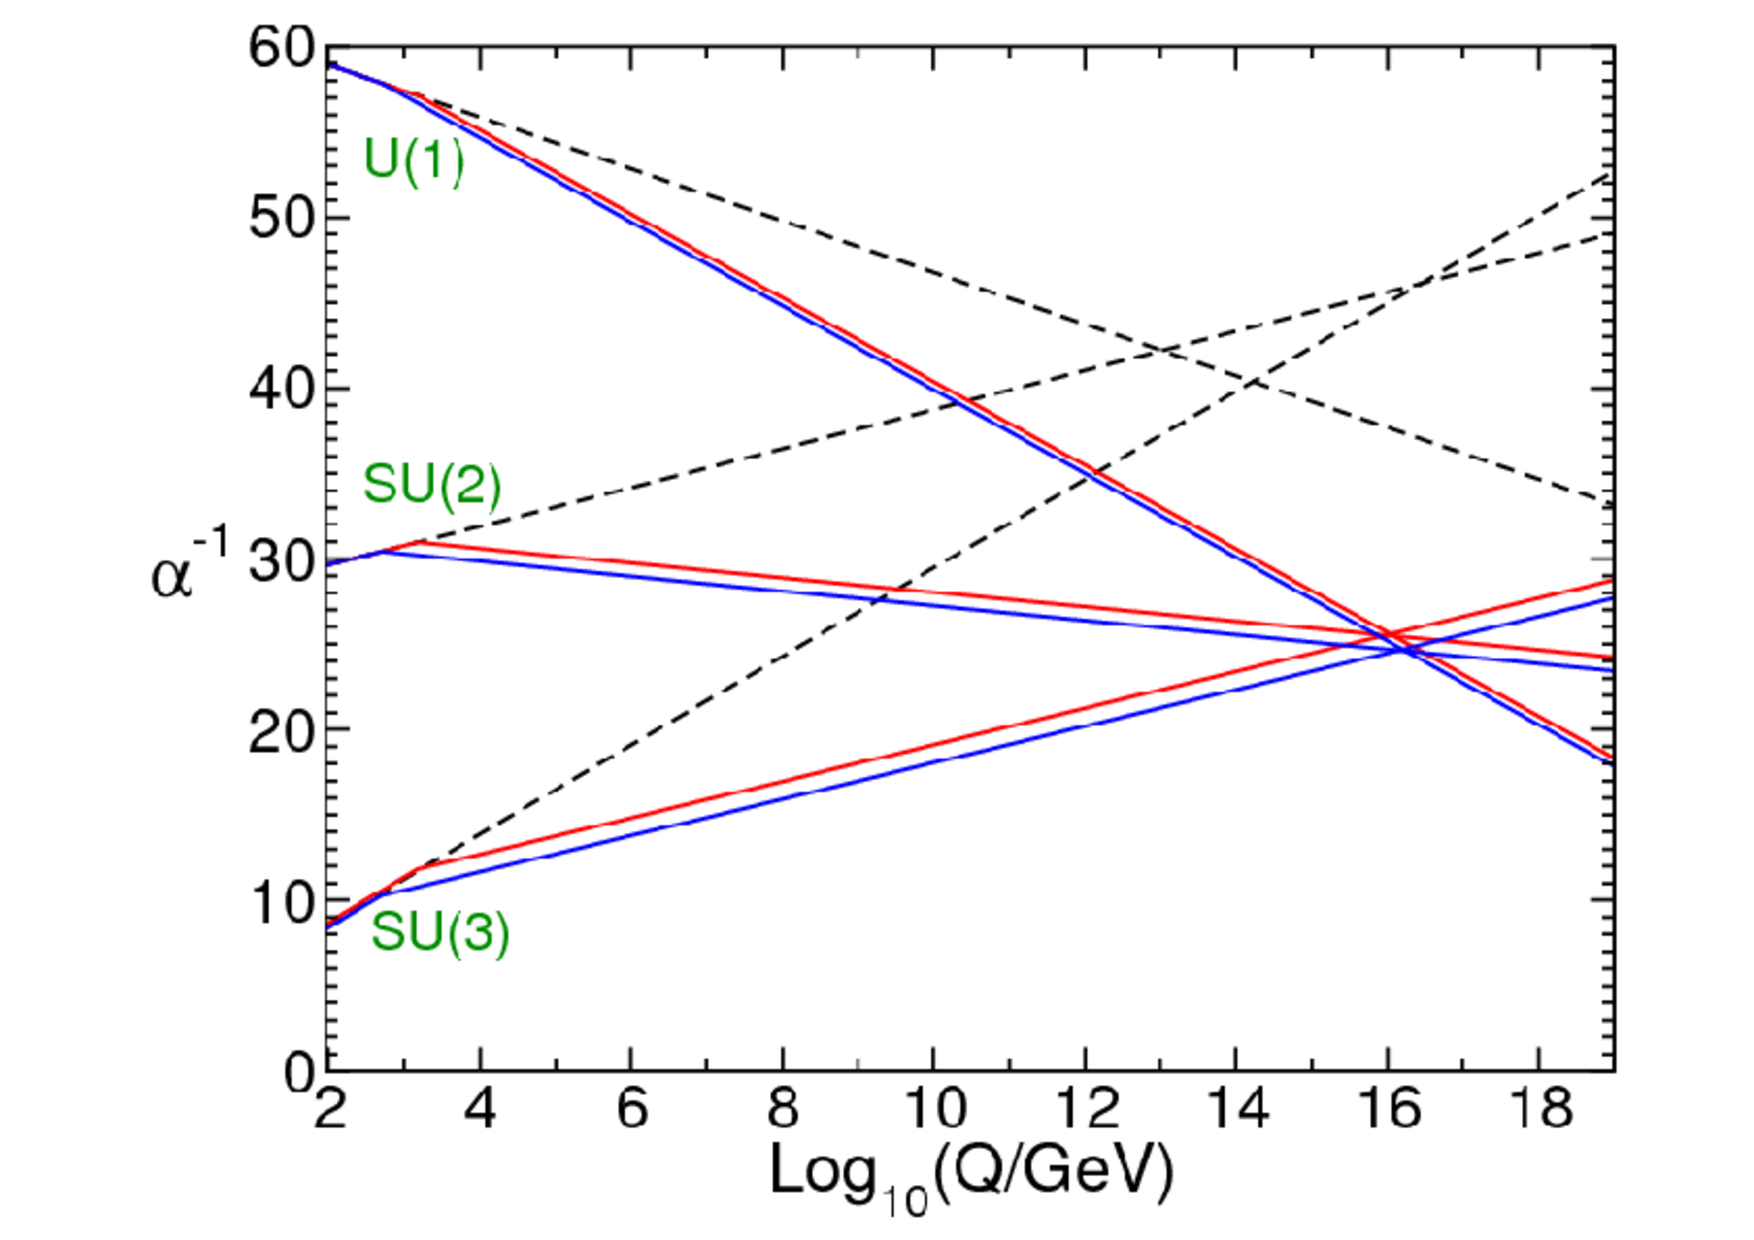
\includegraphics[width=0.7\linewidth]{figures/MSSMGUT.pdf}
\captionof{figure}[Gauge Unification of couplings in the MSSM.]{Renormalization Group Equation (\acrshort{rge}) two-loop evolution of the inverse gauge couplings in the MSSM (solid lines) and SM (dashed lines). The difference in solid lines corresponds to the variation in the weak-scale SUSY threshold and strong coupling constant at $M_Z$. Taken from \cite{RN75}.}
\label{fig:MSSMGUT}
\end{center}

\subsection{The Higgs and electroweakino sector at tree-level}
\label{subsec:MSSMhiggssector}

The full scalar potential, at tree-level, decomposed into the component Higgs fields can be written as:
\begin{equation}
V&=(m^2_{H_u}+|\mu|^2)\left( \left|h^+_{u}\right|^2+\left|h^0_{u}\right|^2 \right) + (m^2_{H_d}+|\mu|^2)\left( \left|h^0_{d}\right|^2+\left|h^-_{d}\right|^2 \right) \nonumber \\
&+B_{\mu}\left( (h^+_u h^-_d - h^0_{u}h^0_{d})+\text{c.c.}\right) \nonumber \\
&+\frac{1}{8}(g^2+g'^2)\left( \left|h^+_{u}\right|^2+\left|h^0_{u}\right|^2-\left|h^0_{d}\right|^2-\left|h^-_{d}\right|^2 \right)^2 +\frac{1}{2}g^2 |h^{0 \dagger}_d h^+_u + h^{- \dagger}_d h^0_u|^2,
\end{equation}
where $g$ and $g'$ are the $\SUgroup{2}_L$ and $\Ugroup{1}_Y$ gauge couplings, respectively. It is immediately apparent that the potential minimizes at $h^-_d = h^+_u = 0$, which is good news as this not being the case would lead to electromagnetism being spontaneously broken, in conflict with experiment. Either way we could have used the $\SUgroup{2}$ freedom to rotate away these component fields in the doublet, but one needs to be sure that this is indeed a minimum first. The potential can then be re-written as
\begin{equation}
V&=(m^2_{H_u}+|\mu|^2)\left|h^0_{u}\right|^2 + (m^2_{H_d}+|\mu|^2)\left|h^0_{d}\right|^2 \nonumber \\
&-B_{\mu}(h^0_{u}h^0_{d}+\text{c.c.})+\frac{1}{8}(g^2+g'^2)\left( \left|h^0_{u}\right|^2-\left|h^0_{d}\right|^2 \right)^2.
\end{equation}
Clearly, the potential is bounded from below since it will be dominated by the quartic terms in $h^0_{u}$ and $h^{0}_{d}$ in the large-field limit. This term vanishes however when $h^{0}_{u}=h^{0}_{d}$ and so leads us to the condition that
\begin{equation}
2B_{\mu}<2|\mu|^2+m^2_{H_u}+m^2_{H_d},
\end{equation}
such that when this is satisfied the potential will rise to positive infinity in all field directions. We typically call the field direction in which $V_{D}$ vanishes the `\textit{D-flat direction}'. Similarly to facilitate electroweak symmetry breaking, we require that the potential be a saddle point at the origin, leading to the second condition
\begin{equation}
(|\mu|^2+m^2_{H_u})(|\mu|^2+m^2_{H_d})<B^2_{\mu}.
\end{equation}
The final two conditions on the parameters of the MSSM relate to the minimization of the potential (vanishing first dervatives \textit{not} at the origin). Let us use the notation $\left\langle h^0_u\right\rangle \equiv v_u$ and $\left\langle h^0_d\right\rangle \equiv v_d$ for the vacuum expectation values.
It will become useful later to make the identifications
\begin{equation}
\tan{\beta}\equiv\frac{v_u}{v_d},\quad v^2=v^2_{u}+v^2_{d},
\end{equation}
where $v$ is equivalent to the SM vacuum expectation value of $v \sim 246$ GeV. Expanding around $\left\langle h^0_u\right\rangle \equiv v_u$ and $\left\langle h^0_d\right\rangle \equiv v_d$, we can compute the physical masses of each of the states from the two Higgs multiplets. We get 3 massless states $m_{\xi^0}=m_{\xi^{\pm}}=0$ that are identified with the Goldstone bosons, which become the longitudinal modes of the $W$ and $Z$ bosons. The masses of the 5 remaining physical Higgs bosons are
\begin{eqnarray}
m^2_{A^0}&=& 2B_{\mu}/\sin {2\beta}, \\
m^2_{h^0,H^0}&=& \frac{m^2_{A^0}+m^2_Z}{2} \mp \frac{1}{2}\sqrt{(m^2_{A^0}+m^2_Z)^2-4m^2_{A^0}m^2_Z \cos^2{2\beta}}, \\
m^2_{H^{\pm}}&=&m^2_W + m^2_{A^0}.
\end{eqnarray}
Interestingly, the mass of the $CP$-odd Higgs boson is unbounded since it scales with $2B_{\mu}/\sin {2\beta}$, and similarly for $H^0$ and $H^{\pm}$, but this is not the case for the lightest Higgs boson $h^0$ which is identified with the Standard Model one. In fact, we get an uncomfortable upper-bound on its mass
\begin{equation}
m_{h^0} < m_Z |\cos {2\beta}|,
\label{eqn:mhtree}
\end{equation}
around the $Z$ boson mass. But this is just the tree-level expression, the sizable one-loop corrections will be discussed in the following section. For now, we are also interested in the electroweakino sector, containing the chargino and neutralino eigenstates. These are important in the calculation of the muon $(g-2)_{\mu}$ and other low-energy predictions of the MSSM, including our prime dark matter candidate. Firstly, the neutralino masses can be computed from the gauge-eigenstate basis $(\Psi^0)^T = (\tilde{B}^0,\tilde{W}^0,\tilde{H}^0_d,\tilde{H}^0_u)$, which contributes to the Lagrangian as
\begin{equation}
\mathcal{L}_{\tilde{\chi}^0}=-\frac{1}{2} (\Psi^0)^T \mathcal{M}_{\tilde{\chi}^0} \Psi^0 + c.c.,
\end{equation}
with the 4 x 4 symmetric matrix
\begin{equation}
\mathcal{M}_{\tilde{\chi}^0}=
\begin{pmatrix}
M_1 &  0 &  -g'v_d/\sqrt2 & g'v_u/\sqrt2 \\ 
 0 &  M_2 & gv_d/\sqrt2 & -gv_u/\sqrt2 \\ 
 -g'v_d/\sqrt2 & -gv_d/\sqrt2 &  0 & -\mu \\ 
 g'v_u/\sqrt2 & -gv_u/\sqrt2 &  -\mu & 0
\end{pmatrix}.
\label{eqn:neutralinoMM}
\end{equation}
This can of course be diagonalized by a unitary matrix $N$ to obtain the mass eigenstates %$\tilde{\chi}^0_i$ $(i=1,2,3,4)$, 
\begin{equation}
N^* \mathcal{M}_{\tilde{\chi}^0} N^{-1} = \text{diag}(m_{\tilde{\chi}^0_1},m_{\tilde{\chi}^0_2},m_{\tilde{\chi}^0_3},m_{\tilde{\chi}^0_4}),
\end{equation}
where $m_{\tilde{\chi}^0_1}<m_{\tilde{\chi}^0_2}<m_{\tilde{\chi}^0_3}<m_{\tilde{\chi}^0_4}$.
Now with this in mind, the lightest mass eigenstate is simply the linear combination of basis states
\begin{equation}
\tilde{\chi}^0_1 = N_{11} \tilde{B}^0 + N_{12} \tilde{W}^0 + N_{13} \tilde{H}^0_d + N_{14} \tilde{H}^0_u.
\end{equation}
Table \ref{tab:LSP} shows that the order of the parameters in Eq. \ref{eqn:neutralinoMM} determines the main component of the neutralino \acrshort{lsp} and \acrshort{nlsp}. This has a dramatic impact on dark matter observables when the LSP is taken to be a dark matter candidate. The charged versions of the electroweakinos, called the charginos, come from the mixing of the $\tilde{W}^{\pm}$ and $\tilde{H}^{\pm}$ eigenstates and can be diagonalized in a similar way.
\begin{table}[]
\captionof{table}[MSSM neutralino hierarchy.]{Hierarchy of the MSSM parameters contributing to the 2 lightest neutralino components.}
\label{tab:LSP}
\centering
\begin{tabular}{|l|l|l|}
\hline
Parameters                                & \textbf{LSP} & \textbf{NLSP} \\ \hline
\textit{$M_1 > M_2 > \mu$}                & Higgsino     & Wino          \\ \hline
\textit{$M_1 > \mu > M_2$}                & Wino         & Higgsino      \\ \hline
\textit{$M_2 > \mu > M_1$}                & Bino         & Higgsino      \\ \hline
\textit{$ \mu > M_2 > M_1$}               & Bino         & Wino          \\ \hline
\end{tabular}
\end{table}

\subsection{The Higgs boson mass at 1-loop}
\label{subsec:MSSMhiggssec}

In the MSSM, we have the contributions to the (lightest) Higgs mass-squared coming from the diagrams shown in Figure \ref{fig:higgscont}, with the largest contribution coming from the large Yukawa coupling of the 3rd generation squarks.
\begin{center}\scalebox{0.62}{
\fcolorbox{white}{white}{
  \begin{picture}(718,136) (51,-139)
    \SetWidth{1.0}
    \SetColor{Black} 
\Line[dash,dashsize=10](128,-104)(192,-104)
\Arc[arrow,arrowpos=0.5,arrowlength=5,arrowwidth=2,arrowinset=0.2](224,-104)(32,270,630)
\Arc[arrow,arrowpos=0.5,arrowlength=5,arrowwidth=2,arrowinset=0.2](224,-104)(32,90,450)
\Line[dash,dashsize=10](256,-104)(320,-104)
\Line[dash,dashsize=10](384,-104)(448,-104)
\Line[dash,dashsize=10](448,-104)(512,-104)
\Arc[dash,dashsize=10](448,-72)(32,270,630)
\Line[dash,dashsize=10](576,-104)(640,-104)
\Arc[dash,dashsize=10](672,-104)(32,270,630)
\Line[dash,dashsize=10](704,-104)(768,-104)
    \Text(352,-108)[lb]{\Large{\Black{$+$}}}
    \Text(544,-108)[lb]{\Large{\Black{$+$}}}
    \Text(448,-24)[lb]{\Large{\Black{$\tilde{t}$}}}
    \Text(672,-56)[lb]{\Large{\Black{$\tilde{t}$}}}
    \Text(224,-56)[lb]{\Large{\Black{$t$}}}
    \Text(90,-108)[lb]{\Large{\Black{$=$}}}
    \Text(48,-108)[lb]{\Large{\Black{$\Delta m^2_{h}$}}}
  \end{picture}
}}
\vspace{10mm}
\captionof{figure}[Higgs boson mass in softly-broken minimal supersymmetry.]{Largest contributions to the lightest Higgs boson mass in softly-broken minimal supersymmetry come from top-quark and stop-squark loop diagrams. Since thefirst two cancel exactly in supersymmetry, the last diagram (corresponding to the second term on the right-hand side of Eq. \ref{eqn:higgsmass}) which is introduced explicitly in soft-supersymmetry breaking, raises the Higgs boson mass by an amount proportional to $\ln{(m_{\tilde{t}}/m_{t})}$.}
\label{fig:higgscont}
\end{center}
In exact supersymmetry at one-loop the first two diagrams in Figure \ref{fig:higgscont} of course cancel, and that is the end of the story. However the presence of soft breaking terms means that the final diagram will contribute to $\Delta m^2_h$ at the order of the supersymmetry breaking scale, typically taken as the geometric mean of the two squark masses, $M_{S}=\sqrt{m_{\tilde{t}_1} m_{\tilde{t}_2}}$. Hence, at one-loop level, the Higgs boson mass has an upper bound of the form
\begin{equation}
m^2_{h} \lesssim m^2_{Z}\cos^2{2\beta}+\frac{3g^2m^4_{t}}{8\pi^2m^2_{W}}\left[\ln{\left(\frac{M^2_{S}}{m^2_{t}}\right)}+\frac{X^2_{t}}{M^2_{S}}\left( 1-\frac{X^2_{t}}{12M^2_{S}}\right)\right],
\label{eqn:higgsmass}
\end{equation}
where $X_{t}\equiv A_{t}-\mu\cot\beta$ represents the off-diagonal stop squark mixing component, which is maximized when $X_{t}=\sqrt{6}M_{S}$, aptly named the "maximal mixing scenario" \cite{RN230}. The tree-level Higgs boson mass coming from the first term saturates at large $\tan \beta$ and so the predicted mass has a lower limit around $m_Z$ without radiative corrections, in tension with experimental observation. Moreover, since experimental searches for stops and other superpartners have shown that these cannot exist at low-energies \cite{RN567,RN568,RN569,RN570}, radiative corrections must then contribute to a net fine-tuning of the Higgs boson mass of a few percent or so. Some have termed this issue 'the little hierarchy problem' in reference to the hierarchy between the electroweak and SUSY breaking scale. Of course this is distinct to the `real' hierarchy problem between the electroweak and Planck scale which is much more severe  - though these are removed completely even in minimal supersymmetry.

\section{Remarks on the MSSM and beyond}

Obviously our introduction of explicit soft supersymmetry breaking terms neglected the consideration of any particular mechanism that communicates this breaking to the MSSM. Naturally this calls for physics beyond the MSSM, some of which we have already mentioned in section \ref{subsec:MSSMsoftbreak}. However, the goal of this thesis is not to explore these various possibilities, but instead to follow what the MSSM as an effective theory is telling us about physics for current energy observables and its behaviour in the UV. Some of the aformentioned issues can even be addressed through simple modification of the MSSM itself, or its place in the evolution of the universe. However, our intention hereforth is now to determine how minimal supersymmetry stacks up with current experimental observations.

